
\RequirePackage{fix-cm}
\documentclass[twocolumn]{svjour3}
\smartqed

\usepackage{cite}
\usepackage[pdftex]{graphicx}
\usepackage{ragged2e}
\usepackage[tight,footnotesize]{subfigure}
\usepackage{rotating}
\usepackage{graphicx}
\usepackage{amsmath,amssymb}
\usepackage{array}
\usepackage{multirow}
\usepackage{colortbl}
\usepackage{amsfonts}
\usepackage{pifont}
\usepackage{xspace}
\usepackage{etoolbox}
\usepackage{overpic}
\usepackage{color}
\usepackage{microtype}

\usepackage{booktabs}
\usepackage{makecell}
\usepackage{threeparttable}
\usepackage{bbding}
\usepackage[numbers]{natbib}
\usepackage{algorithm}
\usepackage{bm}
\usepackage{nicefrac}
\usepackage{microtype}
\usepackage{xcolor}
\usepackage{appendix}
\usepackage{graphicx}
\usepackage{algorithm}
\usepackage{arydshln}
\usepackage{colortbl}
\usepackage{caption}
\usepackage{graphicx}
\usepackage{array}
\usepackage{algpseudocode}

\newcommand{\figref}[1]{Fig.~\ref{#1}}
\newcommand{\tabref}[1]{Table~\ref{#1}}
\newcommand{\equref}[1]{Equ.~(\ref{#1})}
\newcommand{\secref}[1]{\S\ref{#1}}

\newcommand{\orcid}[1]{\href{https://orcid.org/#1}{
\includegraphics[width=10pt]{ocrid.png}}}

\newcommand{\ourDataset}{CDS2K}
\newcommand{\sArt}{state-of-the-art }
\newcommand{\rev}[1]{{\textcolor{red}{#1}}}
\newcommand{\tabincell}[2]{\begin{tabular}{@{}#1@{}}#2\end{tabular}}
\newcommand{\myPara}[1]{\vspace{.15in}\noindent$\bullet$~\textbf{#1}}

\definecolor{myRed}{RGB}{219, 68, 55}
\definecolor{myGreen}{RGB}{15, 157, 88}
\definecolor{myBlue}{RGB}{66, 133, 244}

\newcommand{\tr}[1]{{\textcolor{myRed}{\textbf{#1}}}}
\newcommand{\tg}[1]{{\textcolor{myGreen}{\textbf{#1}}}}
\newcommand{\tb}[1]{{\textcolor{myBlue}{\textbf{#1}}}}

\def\eg{\emph{e.g.}}
\def\ie{\emph{i.e.}}
\def\etc{{\em etc.}}
\def\etal{{\em et al.}}

\definecolor{mygray1}{gray}{.77}
\definecolor{mygray2}{gray}{.92}

\definecolor{CiteColor}{RGB}{0, 113, 188}

\usepackage[breaklinks=true,citecolor=blue, colorlinks]{hyperref}

\graphicspath{{./}}
\DeclareGraphicsExtensions{.pdf,.jpg,.png}


\usepackage{silence}
\hbadness=10000 \vbadness=10000

\definecolor{personcolor}{RGB}{234, 60, 49}
\definecolor{othervehiclecolor}{RGB}{96,81,242}
\definecolor{mygrey}{gray}{0.9}

\newcommand{\mc}[1]{\textcolor{orange}{\textbf{Mingchen:} #1}}
\newcommand{\model}{DreamConnect}


\title{Connecting Dreams with Visual \\Brainstorming Instruction}

\author{
  Yasheng Sun$^{1}$\orcid{0000-0002-5245-7518} \and
  Bohan Li$^{2}$\orcid{0000-0002-5245-7518} \and
  Mingchen Zhuge$^{3}$\orcid{0000-0002-5245-7518}\\
  Deng-Ping Fan$^{4*}$\orcid{0000-0002-5245-7518} \and
  Salman Khan$^{5}$\orcid{0000-0002-5245-7518} \and \\
  Fahad Shahbaz Khan$^{5}$\orcid{0000-0002-5245-7518} \and
  Hideki Koike$^{1}$\orcid{0000-0002-5245-7518}
}

\authorrunning{Sun~\etal}

\institute{
$^1$ CS, Tokyo Institute of Technology, Tokyo 152-8550, Japan. \\
$^2$ CS, Shanghai Jiaotong University, Shanghai 200240, China. \\
$^3$ Center of Excellence for Generative AI, KAUST, Thuwal 23955-6900, Saudi Arabia. \\
$^4$ CS, Nankai University, Tianjin 300350, China. \\
$^5$ CV Group, MBZUAI, Abu Dhabi 20015, UAE. \\
$^*$ Corresponding author: D.-P. Fan (dengpfan@gmail.com)\\
}

\date{Received: date / Accepted: date}


\journalname{}

\begin{document}

\maketitle

\begin{figure*}[h]
  \centering
  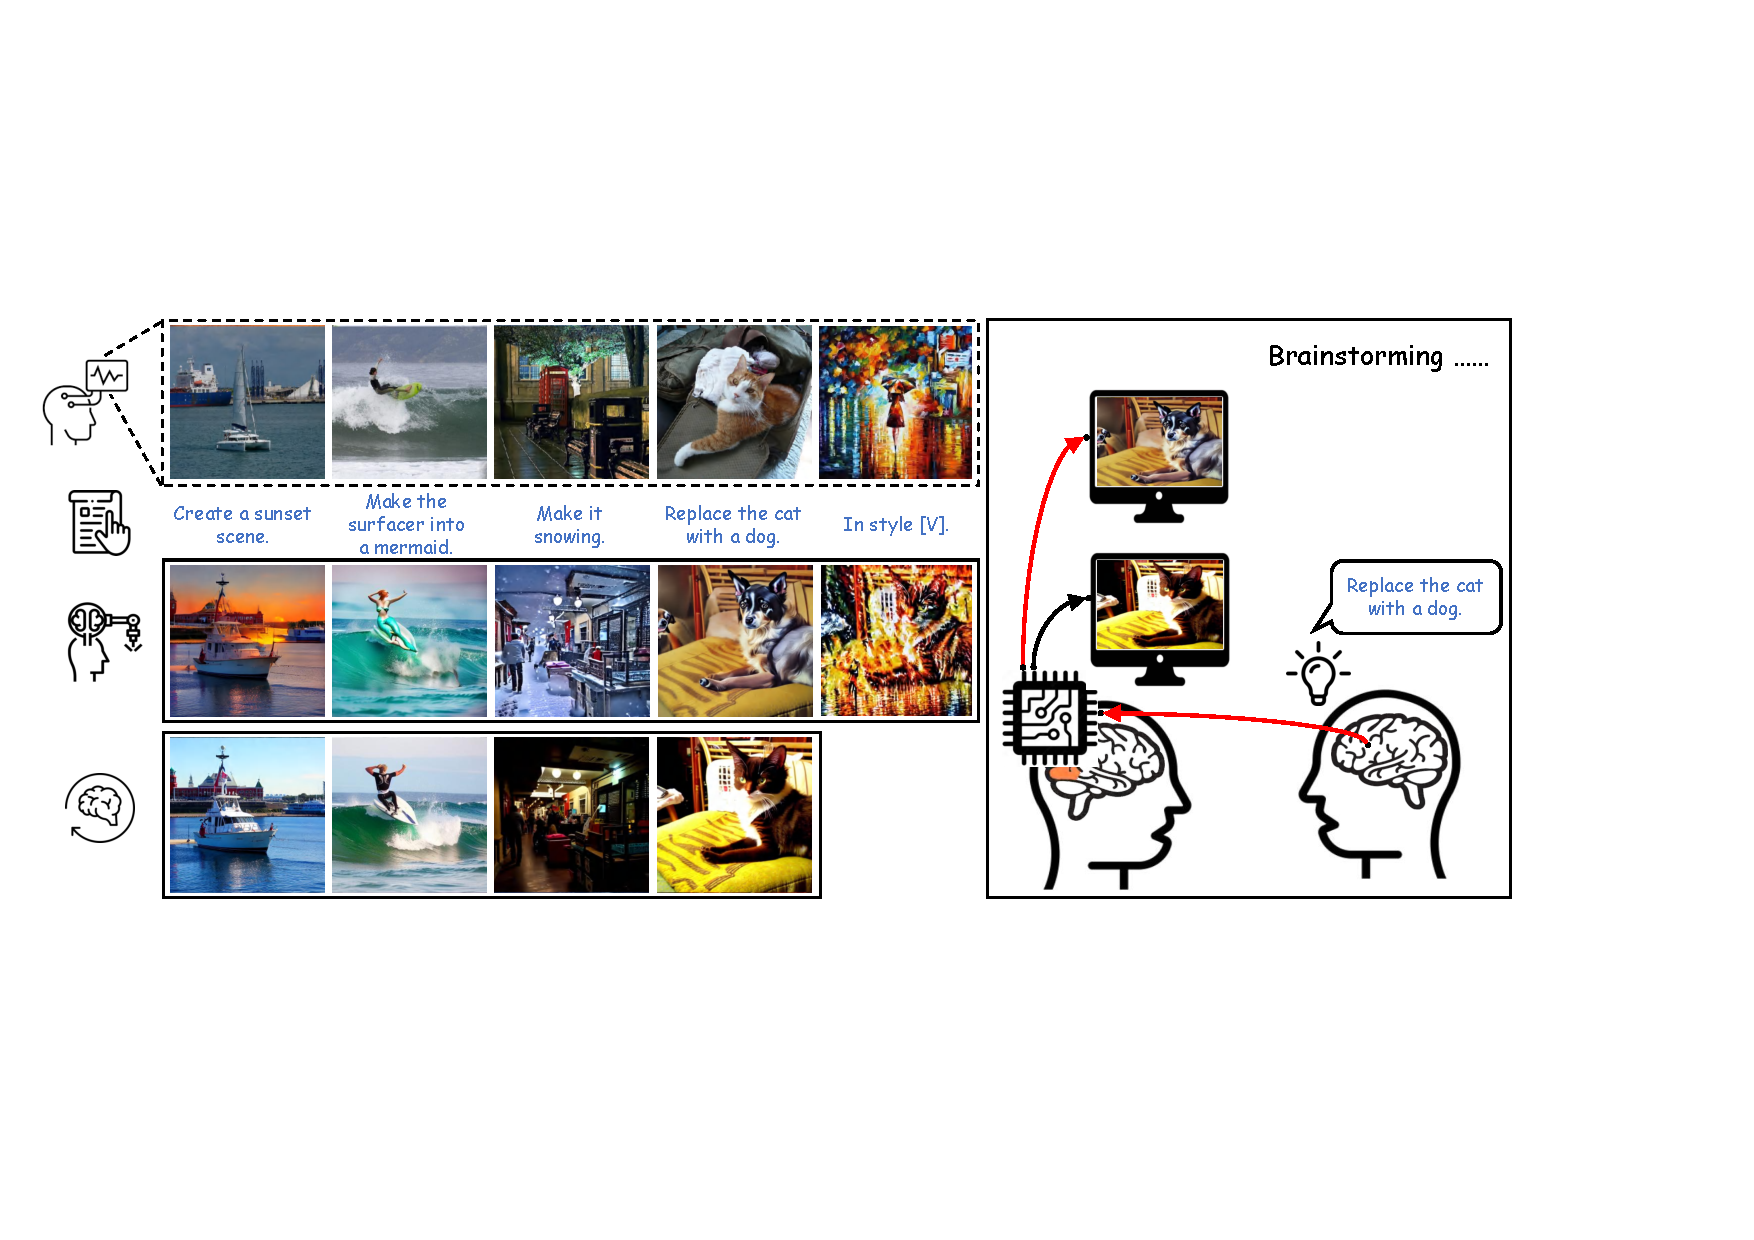
\includegraphics[width=1.0 \textwidth]{figs/teaser1.pdf}
  \caption{\textit{Can dreams be connected and actively influenced in future applications?} As can be seen, \textbf{\model{}} precisely performs the desired operation on the visual content. For example, suppose someone imagines a lake view (see \textbf{the first row}) and another one considers changing it to a sunset scene (\textbf{the second row}). In that case, our system faithfully generates the desired sunset ambiance (\textbf{the third row}).}
  \label{fig:teaser}
\end{figure*}


\begin{abstract}

%Recent advances in understanding human brain activity have revealed its remarkable ability to process and interpret concepts within individuals' minds, providing an efficient way to interface with reality. 
Recent breakthroughs in understanding the human brain have revealed its impressive ability to efficiently process and interpret human thoughts, opening up possibilities for intervening in brain signals.
%However, current methods strongly rely on translating brain signals into another modality as an intermediate step, limiting their usefulness and potentially leading to cumulative errors. 
In this paper, we aim to develop a straightforward framework that uses other modalities, such as natural language, to translate the original ``dreamland''.
%We first provide a more straightforward method, termed as \textbf{\model{}}, 
% which instructs the brain activity signals using natural language description, empowering users to directly tailor their mental imagery. 
%Our approach employs a dual-stream diffusion framework for manipulating visually stimulated brain signals, integrating a multi-scale adaptor and an asynchronous diffusion strategy to fully leverage the underlying diffusion prior for faithful instruction. 
We present \textbf{\model{}}, employing a dual-stream diffusion framework to manipulate visually stimulated brain signals. 
%It integrates a multi-scale adaptor and an asynchronous diffusion strategy to fully leverage the underlying diffusion prior for accurate instruction.
By integrating an asynchronous diffusion strategy, our framework establishes an effective interface with human ``dreams'', progressively refining their final imagery synthesis. 
%To further encourage the model to operate on intended spatial locations, we introduce a Large Language Model (LLM) agent to identify regions pertinent to instructions. 
%Extensive experiments demonstrate the efficacy of our approach in precisely interfacing with brain activity signals, where our framework achieves desired instruction with high identity preservation.
Through extensive experiments, we demonstrate the method's ability to accurately instruct human brain signals with high fidelity. Our project will be publicly available on \textcolor{blue}{\href{https://github.com/Sys-Nexus/DreamConnect}{https://github.com/Sys-Nexus/DreamConnect}}.

\end{abstract}

\keywords{fMRI, Brain-to-Image Generation, Diffusion Models, LLM Agent}



\section{Introduction}
The emergence of deep generative models~\cite{rombach2022high,ho2020denoising,takagi2023high,chen2023seeing,scotti2023reconstructing,lu2023minddiffuser,sun2024contrast,shen2024neuro,xia2024dream} has effectively bridged the modality gap between functional Magnetic Resonance Imaging (fMRI)~\cite{ogawa1990oxygenation} and diverse signals like visual, language, and audio.
However, many studies~\cite{,bai2023dreamdiffusion,lan2023seeing,zeng2023controllable,vanrullen2019reconstructing,dado2022hyperrealistic,shen2019deep,seeliger2018generative,NEURIPS2022_bee5125b,gu2022decoding,liu2024mind} focus on recovering the stimulated signal from brain activity, while interaction with reality requires active communication with human brain signals.

In this work, we explore a novel setting as shown in Fig.~\ref{fig:teaser} -- \emph{Can ``dreams'' be connected and actively influenced?} Such capability will present a novel and convenient interaction paradigm among people, facilitating numerous applications such as creative design via brainstorming.
The essence of this capability lies in steering the human ``dreams'' towards desired directions, ultimately \emph{enabling concept manipulation through direct operation on the fMRI signal}.
This paper mainly focuses on human ``dreams'' as a visual modality, but the fMRI signal can also store other types of stimulated information, such as audio~\cite{defossez2023decoding} or language~\cite{zhao2024mapguide}. Consequently, our proposed approach can be seamlessly extended to these scenarios.


This task requires direct instruction of fMRI signals, which presents notable challenges on two fronts: 1) The inherent abstractness and ambiguity of collected brain signals often impede the comprehension of their content;
2) A significant modality gap exists between fMRI signals and natural language instructions, hindering the learning of accurate associations between brain activity features and language instructions. Since not all the information within the fMRI signals is relevant to the intended instruction, successful instruction requires \emph{pinpointing and modifying the relevant features while preserving the irrelevant ones}.



We introduce \textbf{\model{}}, a dual-stream diffusion framework tailored for fMRI signal instruction to address these challenges. The key is to \emph{effectively guide language instructions to hone in on and modify the pertinent information embedded within fMRI signals}. To establish a correlation between these distinct signals, we first employ a Stable Diffusion (SD)~\cite{rombach2022high} backbone to interpret brain activity using visual prior knowledge. Then, we integrate language instructions into a parallel SD backbone to manipulate the acquired visual priors.
This parallel forwarding approach has proven to be effective in improving network learning ability by leveraging the homogeneous nature of the extracted features~\cite{zhang2023adding}. To bridge these two streams, i.e., the interpretation stream and instruction stream, we introduce an adaptor network designed to modulate the intermediate visual contents from the interpretation stream hierarchically.

Ideally, with this design, the framework will operate under a \emph{progressive interpretation and instruction paradigm, concurrently identifying and manipulating correlated regions}. However, the diffusion operation behaves distinctively along the temporal dimension, synthesizing varied content across different time steps~\cite{zhang2023prospect,Zhang_2023_inst}. At specific time steps, the second stream must identify specific visual features for instruction, necessitating that the first stream completes their formation beforehand. Therefore, we devise an asynchronous diffusion strategy to ensure that the first stream has adequate time to develop overall semantics, thereby facilitating smooth manipulation progress. Additionally, to further guide the model toward intended spatial locations, we introduce a Large Language Model (LLM)~\cite{wei2022emergent} agent tasked with identifying regions relevant to instructions. Using the identified areas, we implement a region-aware attention strategy to ensure that the instructions are applied precisely within those regions.
\textbf{Our main contributions can be summarized as:}

\noindent \textbf{(1)} We propose a visual brainstorming instruction system, named \textbf{\model{}}, empowering users to effectively interfacing with human ``dreams'' to perform desired operation.

\noindent \textbf{(2)} We devise a dual-stream diffusion network coupled with an adaptor to seamlessly translate fMRI signals towards their intended directions.

 \noindent \textbf{(3)} We introduce an asynchronous diffusion strategy, enhanced with LLM-guided region-aware manipulation, to facilitate faithful instruction within pertinent regions from both temporal and spatial perspectives.
\noindent \textbf{(4)} While designed for language-guided instruction, our framework can readily adapt to visual instruction or multi-modal instruction with minimal adjustments.




\section{Related Work}


\noindent \textbf{Brain Activity Recognition.}
Earlier studies~\cite{vanrullen2019reconstructing,dado2022hyperrealistic,shen2019deep,seeliger2018generative,NEURIPS2022_bee5125b,gu2022decoding,ferrante2022semantic} aimed to reconstruct visual stimuli by decoding brain signals into the latent space of Generative Adversarial Networks~\cite{goodfellow2020generative}. Given the significant capabilities of diffusion models in image generation~\cite{rombach2022high,ho2020denoising}, numerous investigations~\cite{takagi2023high,chen2023seeing,scotti2023reconstructing,lu2023minddiffuser,bai2023dreamdiffusion,lan2023seeing,zeng2023controllable,li2024neuraldiffuser,fang2024alleviating,li2024visual} have explored the use of their image prior for high-quality reconstruction. To improve reconstruction performance, some studies~\cite{zeng2023controllable,lu2023minddiffuser} exploit low-level signals within fMRI to achieve spatially consistent predictions by imposing spatial constraints during the generation process. Another set of studies~\cite{liu2023brainclip} has sought to leverage contrastive learning, such as CLIP, to improve semantic alignment in reconstruction. Certain works demonstrate the effectiveness of masked pretraining~\cite{he2022masked,bai2023dreamdiffusion} of brain signals on large datasets, facilitating robust latent space learning.
Moreover, novel applications related to brain activity~\cite{sun2023tuning,sun2024neurocine,wang2024mindbridge,nikolaus2024modality,xia2024umbrae,chen2024bridging,huo2024neuropictor} have emerged. For instance, Mind-Video~\cite{chen2023cinematic} extends image reconstruction to video reconstruction, while UniBrain~\cite{mai2023unibrain} not only reconstructs visual signals but also generates corresponding captions.

\paragraph{Image Manipulation.}
With a plethora of diverse generative priors embedded within powerful diffusion architectures, numerous studies~\cite{avrahami2023blended,couairon2022diffedit,meng2021sdedit,nichol2021glide,sun2023imagebrush,sun2024avi} have endeavored to adapt them for image manipulation. To facilitate the editing of desired semantic regions within spatial feature maps, researchers have proposed various techniques such as cross-attention injection~\cite{hertz2022prompt,balaji2022ediffi} and introduced semantic loss~\cite{tumanyan2023plug} to constrain spatial features during the generation process. Additionally, to provide explicit guidance towards intended instructions, subsequent works~\cite{brooks2023instructpix2pix,geng2023instructdiffusion} leverage language-based instructions to fine-tune the SD model, showcasing impressive capabilities in conforming to desired editing directions.
However, these approaches primarily operate on raw images. Few have delved into manipulating stored visual content with another modality, which holds potential for diverse applications such as fostering friendly human-computer interaction.

\paragraph{LLM Agent For Visual Assistance.}
Large language models (LLMs) have showcased profound capabilities as remarkable reasoning engines in various tasks~\citep{zhuge2023mindstorms,wei2022chain,huang2022towards,Touvron2023LLaMAOA,brown2020language}, due to their emerging ability~\citep{wei2022emergent}.
With rich contextual prior knowledge, LLMs adeptly tackle a multitude of visual-language tasks~\citep{zhuge2024language,alayrac2022flamingo,zhang2023multimodal,chakrabarty2023spy} via appropriate prompting adaptation.
Through visual instruction tuning, LLMs can discern image content, reason about involved events, and generate plausible responses~\citep{li2023blip,liu2024visual,zhu2023minigpt}. Subsequent studies~\citep{koh2024generating,sun2023generative,wu2023visual} have shown that LLMs can naturally provide visual feedback by leveraging an image rendering backbone such as a diffusion model.
Recently, researchers have employed LLMs to facilitate the image generation process~\citep{NEURIPS2023_3a7f9e48,fu2023guiding}, where the language model exhibits impressive capabilities in layout reasoning and instruction execution.

\section{Methodology}

\begin{figure*}[t!]
  \centering
   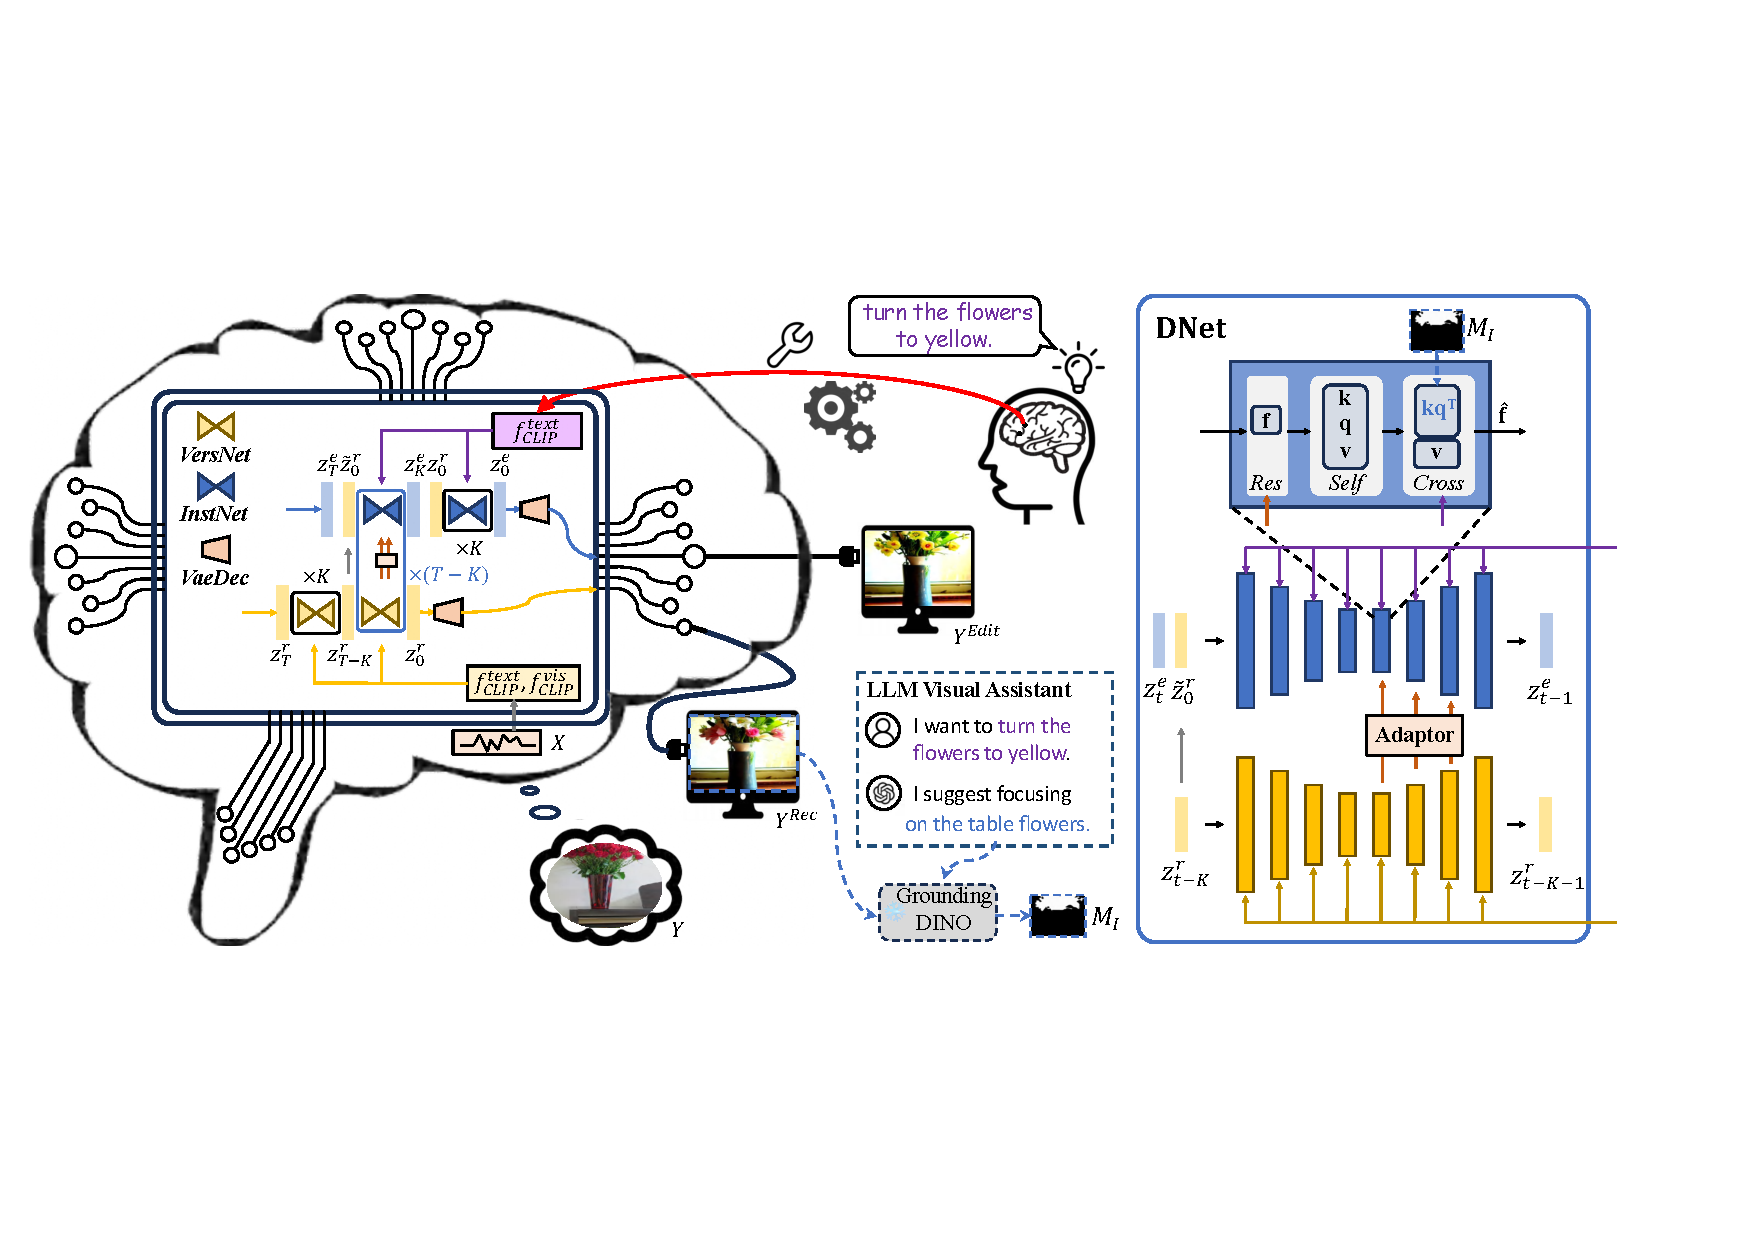
\includegraphics[width=\linewidth]{figs/arch5.pdf}
  \caption{\textbf{Illustration of the proposed \textbf{\model{}} framework.}
    A person's biological signal indicated by fMRI sequences $X$, will be activated within his brain according to his ``dreams'' represented by the visual stimuli $Y$.
    Our system targets to interface with $X$ via a natural language instruction $I$.
    Specifically, the fMRI signal is regressed to CLIP text and visual embedding, $f_{\text{CLIP}}^{text}$ and $f_{\text{CLIP}}^{vis}$, which are leveraged to aligned with visual content $z^r_t$ in \emph{\textbf{VersNet}}~\cite{xu2023versatile}. After modulated by an adaptor, its intermediate spatial features are fed to \emph{\textbf{InstNet}}~\cite{geng2023instructdiffusion}. Encoded by CLIP text encoder, the human instruction $I$ is injected to \emph{\textbf{InstNet}} to modulate these features toward intended direction.
  }
  \label{fig:arch}
\end{figure*}



In this section, we discuss the details of the proposed \emph{Visual Brainstorming Instruction System}, termed \textbf{\model{}}. The primary objective of this framework is to develop a model capable of providing instruction in brain activity. To achieve this, the model must possess the ability to associate human instructions with fMRI signal and modify its embedded pertinent visual information. The overall pipeline is depicted in Fig.~\ref{fig:arch} where we devise an asynchronous dual-stream diffusion architecture coupled with an adaptor to promote \emph{progressive interpretation and instruction}. To facilitate faithful instruction within pertinent regions from both temporal and spatial perspectives, we introduce an asynchronous diffusion strategy and an LLM-guided region-aware manipulation operation.

\subsection{Dual Stream Diffusion Instruction}
\textbf{Problem Formulation.} Given a visual stimuli $Y \in \mathcal{R}^{3 \times H \times W}$, a person's biological signal revealed by fMRI, $X \in \mathcal{R}^{N_f}$, will be activated, where ${N_f}$ represents the number of relevant voxels. The traditional image reconstruction task targets to recover its indicted visual content $Y^{Rec}$ from $X$. In contrast, we study directly manipulating the entailed information to $Y^{Edit}$ following a piece of natural language instruction $I$.
Accomplishing this objective requires a comprehensive cross-modal association between the fMRI signal and the specified instruction. To resolve this issue, we leverage the rich contextual prior within StableDiffusion (SD) to bridge the modality gap due to its effective exploitation in numerous visual tasks. The key is to derive a unified diffusion framework to tackle feature alignment and interaction among distinct modalities progressively.

\paragraph{Preliminary on Diffusion Models.}
Diffusion models~\cite{ho2020denoising} stand out due to its stable training objective and exceptional ability to generate high-quality images. It operates by iteratively denoising Gaussian noise to produce the image $\bm{x}_0$.
Typically, the diffusion model assumes a Markov process~\cite{rabiner1989tutorial} wherein Gaussian noises are gradually added to a clean image $\bm{x}_0$ based on the following equation:
\begin{equation}
    \bm{x}_t = \sqrt{\alpha_t} {\bm{x}}_{0} + \sqrt{1-\alpha_t} \bm{\epsilon} ,
\label{eq:forward}
\end{equation}
where $\bm{\epsilon}\!\sim\!\mathcal{N}(0, \mathbf{I})$ represents the additive Gaussian noise, $t$ denotes the time step and $\alpha_t$ is scalar functions of $t$.
Our objective is to devise
a neural network $\bm{\epsilon}_\theta(\bm{x}_t, t, c)$ to predict the added noise $\bm{\epsilon}$.
Empirically, a simple mean-squared error is leveraged as the loss function:
\begin{equation}
    L_{simple} := \mathbb{E}_{\bm{\epsilon} \sim \mathcal{N}(0, \mathbf{I}), \bm{x}_0, c}\Big[ \Vert \bm{\epsilon} - \bm{\epsilon}_\theta(\bm{x}_{t}, c) \Vert_{2}^{2}\Big] \, ,
    \label{eq:LDM_loss}
\end{equation}
where $\theta$ represents the learnable parameters of our diffusion model, and $c$ denotes the conditional input to the model.
To improve the computational efficiency, latent diffusion models (LDM)~\cite{rombach2022high} proposes to operate in a lower-dimensional latent space that encodes $\bm{x}_t$ to $\bm{z}_t$ through VAE~\cite{esser2021taming}.

\paragraph{Dual Stream Diffusion Network.} The overall synthesis process is visualized in Fig.~\ref{fig:arch}. Given a sequence of fMRI signal $X \in \mathcal{R}^{N_f}$ and a sentence of instruction $I$ such as \emph{turn the flowers to yellow}, our objective is to translate $X$ to $Y^{Edit}$ according to the provided instruction.
The $N_f$ denotes the feature length of collected fMRI signal.
To connect instruction description with fMRI signal, we devise a dual-stream diffusion network for progressive \emph{interpretation and instruction} as shown in the right side of Fig.~\ref{fig:arch}.
Accepting information from fMRI signal, the bottom stream aims to hallucinate visually appealing and semantically consistent content for faithful interpretation of the brain signal.
On top of this stream, another stream  aims to manipulate its decoded visual content according to user-specified instructions. Conditioned on brain signal $X$ and instruction $I$, the dual-stream diffusion network denoises the VAE latent codes $\textbf{z}_t^r$ and $\textbf{z}_t^e$ at each time step $t$. Formally,
\begin{equation}
    [\textbf{z}_{(t-1)}^r, \textbf{z}_{(t-1)}^e] = \textbf{\text{DNet}}_{t}([\textbf{z}_t^r, \textbf{z}_t^e]; I, X).
\end{equation}


For the purpose of bridging visual content and brain activity signal, we choose VersatileDiffusion (VD)~\cite{xu2023versatile} as the bottom-stream backbone because both image and text condition are taken into consideration following typical fMRI-based reconstruction works~\cite{ozcelik2023brain,scotti2023reconstructing}.
Specifically, the UNet of VD adaptively exploit extracted features from CLIP image and text encoder through cross attention.
We leverage their pretrained parameters to initialize the UNet, thereby keeping most generative image prior.
Then the UNet is freezed and we devise a mixed mapping strategy to predict both CLIP text and visual embed, $f_{\text{CLIP}}^{text}$ and $f_{\text{CLIP}}^{vis}$, within a diffusion paradigm.
The mapping network architecture and training strategy adopts align-before-predict paradigm with previous work~\cite{ramesh2022hierarchical,scotti2023reconstructing} but we operates on both visual and text space that co-manipulates VD in a mixed manner.

With the interpreted visual content, upper stream targets to guide them towards the desired instruction direction. A natural way to address this is to inject the CLIP text embedding of the instruction $I$ via cross attention, which is leveraged to modulate the spatial features within a diffusion UNet backbone. To connect these two streams, an adaptor network is introduced to adjust the intermediate features of interpreted visual content for better instruction. The adjusted features are injected only in the decoder part of the UNet due to its clear layout and semantic feature construction~\cite{zhang2023adding}.
To maintain high consistency over the generated shape and layout, we propose to modify the features within residual blocks~\cite{tumanyan2023plug}. To further enhance control over the aligned visual content, we also incorporate the obtained VAE latent $\textbf{z}_t^r$ from bottom stream as concatenation of our input. Note that we convert $\textbf{z}_t^r$ at time $t$ to its denoised estimation $\tilde{\textbf{z}}_0^r$ at time step $t=0$ for consistent representation. Formally,
\begin{equation}
    \tilde{\textbf{z}}_0^r = (\textbf{z}_t^r - \sqrt{1-\overline{\alpha}_t} \bm{g}_{\theta} (\textbf{z}_t^r)) / \sqrt{\overline{\alpha}}_t,
\end{equation}
where the $\overline{\alpha}_t := \prod_{s=1}^t \alpha_s$ increases along with $t$ and $\bm{g}_{\theta}$ indicates the network of bottom stream.
For this stream, we initialize it with pretrained UNet from InstructDiffusion~\cite{geng2023instructdiffusion}.

\subsection{Faithful Instruction via Feature Exploitation}
The core of our framework lies on bridging fMRI signal and language instruction with visual modality. Thus fully utilization of the visual information plays a crucial role in successful instruction. We aim to make most of them from both temporal and spatial perspectives to facilitate faithful instruction.
\paragraph{Asynchronous Diffusion Strategy.} One issue of above strategy is that the aligned visual feature $\textbf{z}_t^r$ might not well prepared for manipulation at time step $t$. This problem becomes more severe especially at early stages because its semantic feature is not well formed, which brings difficulty for the instruction to identify pertinent areas to be edited. To address this, we propose an asynchronous approach where the instruction stream is enforced to lag behind the first stream for $K$ steps. Such practice will offer the first stream sufficient time to develop overall layout or shape semantics. Therefore, the improved version of diffusion process can be written as
\begin{equation}
    [\textbf{z}_{(t\textcolor{red}{-K}-1)}^r, \textbf{z}_{(t-1)}^e] = \textbf{\text{DNet}}_{t}([\textbf{z}_{t\textcolor{red}{-K}}^r, \textbf{z}_t^e]; I, X).
\end{equation}
The $K$ represents the number of time steps that the instruction stream lags behind, which we empirically adopt $K=15$ in our experiment.

\paragraph{LLM-Guided Region-Aware Instruction.} The asynchronous strategy implicitly provides higher chances for user instructions to operate on the appropriate regions. This inspires us to seek mechanisms to explicitly restrict feature manipulation within desired regions. Given the robust reasoning capabilities of LLMs, we leverage them as agents to aid in specifying the intended editing region. As depicted in lower part of Fig.~\ref{fig:arch}, we provide the instruction information to the language model and inquiry for the locations that requires focusing on.
With the obtained advice, we employ it as an text prompt to guide the \emph{Grounding DINO} model to identify the pertinent spatial areas $M^I$ of the reconstructed image $Y^{Rec}$. Then the mask $M_I$ is used to restrict cross-attention. For each cross-attention layer, the instruction features are projected into context values $\textbf{v}$ and keys $\textbf{k}$ while visual features are projected into queries $\textbf{q}$. Its output of this block is given by
\begin{equation}
    \hat{\textbf{f}} = \textbf{A} \textbf{v} \text{  where  } \textbf{A} = \text{Softmax}(\textbf{q}\textbf{k}^T).
\end{equation}
Intuitively, the attention map $\textbf{A}$ determines distribution ratio of context features.
Here the instruction irrelevant region is expected to be untouched. A natural way is to mask out those features outside of $M_I$ by replacing them with attention maps activated by null instruction. Formally,
\begin{equation}
    \textbf{A}_M = \textbf{A}_I M_I + \textbf{A}_{null} (1-M_I)
\end{equation}
where the updated attention map $\textbf{A}_M$ is a masked combination of attention maps activated by instructions and null instructions, $\textbf{A}_I$ and $\textbf{A}_{null}$, respectively. The guiding mask $M_I$ is interpolated to the spatial size of each UNet block.


% \section{Experiments}
\section{实验}

\begin{figure*}[t!]
  \centering
  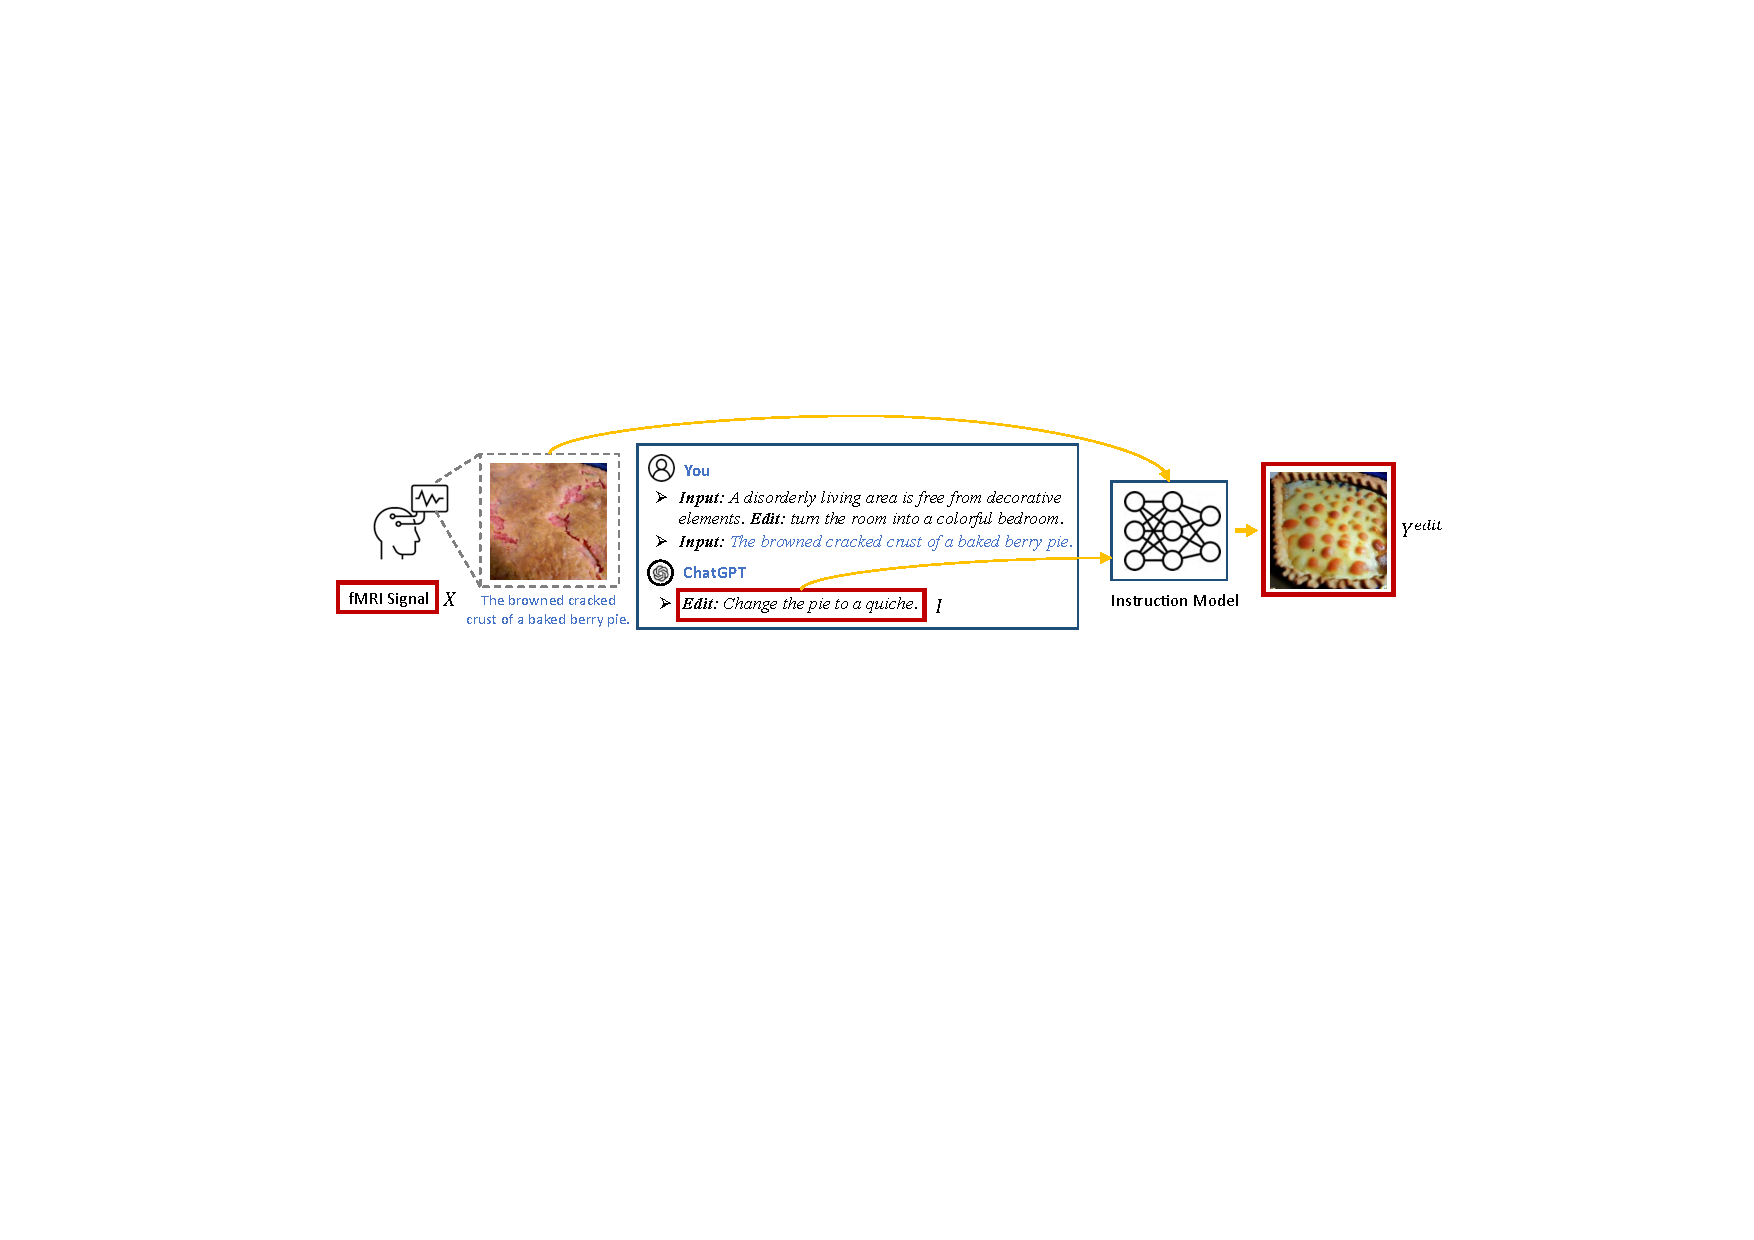
\includegraphics[width=.98\linewidth]{figs/data_pipeline2.pdf}
%   \caption{\textbf{Illustration of Dataset Pipeline.}
%   Given the paired fMRI signal $X$ and its corresponding visual stimuli $Y$ in NSD~\cite{allen2022massive}, we first query LLMs with image caption to obtain possible instruction $I$. Then the instruction, coupled with visual stimuli, is utilized prompt a visual instruction model for manipulated image $Y^{edit}$.
%   Finally, the triplets of $(X, I, Y^{edit})$, are constructed (red boxes).
%   }
  \caption{\textbf{数据集流水线图解。}
  给定 NSD 数据集~\cite{allen2022massive} 中成对的 fMRI 信号 $X$ 及其对应的视觉刺激 $Y$，我们首先利用图像描述查询大语言模型（LLM），以获取可能的指令 $I$。然后，将该指令与视觉刺激结合，用于提示视觉指令模型生成被操纵的图像 $Y^{edit}$。最后，构建出 $(X, I, Y^{edit})$ 三元组（如红框所示）。
  }
  \label{fig:data_pipeline}
\end{figure*}

% \textbf{Datasets.} To validate our proposed approach, we leverage the NSD~\cite{allen2022massive} dataset, the largest neuro-imaging dataset containing densely sampled fMRI data.
\textbf{数据集。} 为了验证我们提出的方法，我们采用了 NSD~\cite{allen2022massive} 数据集，这是目前包含密集采样 fMRI 数据的最大神经成像数据集。
% Participants are asked to view 9000-10000 different pictures over 30-40 MRI scanning sessions.
参与者被要求在 30 到 40 次 MRI 扫描阶段内观看 9000 到 10000 张不同的图片。
% These images are extracted from COCO dataset~\cite{lin2014microsoft}, and corresponding captions are also available. In our experiments, we choose subject 1 from NSD.
这些图像提取自 COCO 数据集~\cite{lin2014microsoft}，并附有相应的描述文本。在我们的实验中，我们选择了 NSD 数据集中的受试者 1（subject 1）。
% For each subject, a total of 9841 image stimuli are presented, with 982 images set aside for validation.
对于每位受试者，共呈现 9841 张图像刺激，其中 982 张图像被留作验证集。
% In our setting, we require triplets of fMRI data, instructions and edited images to train and evaluate our model.
在我们的设定中，我们需要由 fMRI 数据、指令和编辑后图像组成的三元组来训练和评估我们的模型。
% Since such a dataset does not exist, we augment the NSD dataset using Large Language Models (LLMs), as illustrated in Fig.~\ref{fig:data_pipeline}. Specifically, LLMs generate instructions, while a pre-trained visual instruction model accounts for obtaining corresponding edited image.
由于目前不存在这样的数据集，我们利用大语言模型（LLM）对 NSD 数据集进行了扩充，如图~\ref{fig:data_pipeline} 所示。具体而言，LLM 生成指令，而预训练的视觉指令模型负责获取相应的编辑后图像。
% For easy access, we utilize text-davinci-003 engine of ChatGPT~\cite{brown2020language} for in-context instruction synthesis and instructDiffusion~\cite{geng2023instructdiffusion} for visual instruction. Replacing these with more advanced models such as GPT-4V(ison)~\cite{openai2023gpt} or DALL·E 3~\cite{openai2023dalle3} could further improve the dataset quality.
为便于实现，我们利用 ChatGPT~\cite{brown2020language} 的 text-davinci-003 引擎进行上下文指令合成，并使用 instructDiffusion~\cite{geng2023instructdiffusion} 进行视觉指令操作。将这些模型替换为更先进的模型（如 GPT-4V(ision)~\cite{openai2023gpt} 或 DALL·E 3~\cite{openai2023dalle3}）有望进一步提高数据集的质量。

% \paragraph{Implementation. } During the training stage, we freeze the UNet backbones of both the first and second streams to fully leverage the visual priors pre-trained. The overall training process is divided into two stages.
\paragraph{实现细节。} 在训练阶段，我们冻结了第一流和第二流的 UNet 骨干网络，以充分利用预训练的视觉先验。整个训练过程分为两个阶段。
% In the first stage, we target to translate fMRI signal into the visual domain by regressing the intermediate features of CLIP vision/text embedding. The architecture of the regression network and the training paradigms follow protocols similar to MindEye~\cite{scotti2023reconstructing}.
在第一阶段，我们的目标是通过回归 CLIP 视觉/文本嵌入的中间特征，将 fMRI 信号转换到视觉领域。回归网络的架构和训练范式遵循与 MindEye~\cite{scotti2023reconstructing} 相似的协议。
% Once the parameters of this stream have been trained, they are frozen. The adaptor that bridges two streams is finetuned using our extended synthesized dataset.        
一旦该流的参数训练完毕，它们将被冻结。连接这两个流的适配器则使用我们扩展合成的数据集进行微调。
% We employ the Mean Squared Error (MSE) Loss~\cite{ho2020denoising} typical in diffusion models as our optimization objective.
我们采用扩散模型中典型的均方误差（MSE）损失~\cite{ho2020denoising}作为优化目标。
% Since each image stimulus includes three trials, a total of 24980 trials and 8859 visual stimuli are involved in the training set. For fMRI data with multiple trials, we average their responses for consistency.
由于每个图像刺激包含三次试验（trials），训练集中共涉及 24980 次试验和 8859 个视觉刺激。对于包含多次试验的 fMRI 数据，我们对其响应取平均值以保持一致性。
% For our framework and all the compared models, we set the classifier-free scale to 7.5 for image instruction.
对于我们的框架及所有对比模型，在进行图像指令操作时，我们将无分类器引导尺度（classifier-free scale）设置为 7.5。
% Our models are implemented in PyTorch~\cite{paszke2019pytorch} and trained using 80G Tesla A100 GPUs.
我们的模型在 PyTorch~\cite{paszke2019pytorch} 中实现，并使用 80G 的 Tesla A100 GPU 进行训练。

% \paragraph{Comparisons.} Although our framework is designed for fMRI signal instruction, it also supports basic function of reconstruction. Therefore, we validate our method from both the reconstruction and the instruction perspectives.
\paragraph{对比方法。} 尽管我们的框架是为 fMRI 信号指令而设计的，但它也支持基本的重建功能。因此，我们从重建和指令两个视角对我们的方法进行验证。
% For image reconstruction, we compare our method with the best models currently available that support fMRI-based image reconstruction: Takagi \emph{et.al.}~\cite{takagi2023high}, UniBrain~\cite{mai2023unibrain}, Brain-Diffuser~\cite{ozcelik2023brain} and MindEye~\cite{scotti2023reconstructing}.
在图像重建方面，我们将我们的方法与目前支持基于 fMRI 图像重建的最佳模型进行了比较：Takagi \emph{et.al.}~\cite{takagi2023high}、UniBrain~\cite{mai2023unibrain}、Brain-Diffuser~\cite{ozcelik2023brain} 和 MindEye~\cite{scotti2023reconstructing}。
% Takagi \emph{et.al.}~\cite{takagi2023high} pioneered the utilization of image priors from Stable Diffusion (SD)~\cite{esser2021taming} for fMRI-based image reconstruction.
Takagi \emph{et.al.}~\cite{takagi2023high} 开创了利用稳定扩散（SD）~\cite{esser2021taming}图像先验进行基于 fMRI 图像重建的先河。
% UniBrain~\cite{mai2023unibrain} demonstrates the capability to translate fMRI signals to both image captions and images simultaneously.
UniBrain~\cite{mai2023unibrain} 展示了将 fMRI 信号同时转换为图像描述和图像的能力。
% Brain-Diffuser~\cite{ozcelik2023brain} and MindEye~\cite{scotti2023reconstructing} showcase the effectiveness of mapping to CLIP space in the VersatileDiffusion~\cite{xu2023versatile} setting.
Brain-Diffuser~\cite{ozcelik2023brain} 和 MindEye~\cite{scotti2023reconstructing} 展示了在 VersatileDiffusion~\cite{xu2023versatile} 设定下映射到 CLIP 空间的有效性。
% For instruction, we compare our method with state-of-the-art image manipulation approaches, including SDEdit~\cite{meng2021sdedit}, InstructPix2Pix~\cite{brooks2023instructpix2pix}, InstructDiffusion~\cite{geng2023instructdiffusion} and MagicBrush~\cite{zhang2024magicbrush}.
在指令方面，我们将我们的方法与最先进的图像操纵方法进行了比较，包括 SDEdit~\cite{meng2021sdedit}、InstructPix2Pix~\cite{brooks2023instructpix2pix}、InstructDiffusion~\cite{geng2023instructdiffusion} 和 MagicBrush~\cite{zhang2024magicbrush}。
% SDEdit~\cite{meng2021sdedit} proposes to edit image with Stochastic Differential Equation (SDE).
SDEdit~\cite{meng2021sdedit} 提出利用随机微分方程（SDE）来编辑图像。
% InstructPix2Pix~\cite{brooks2023instructpix2pix} directly trains a Stable Diffusion model conditioned on instructions. InstructDiffusion~\cite{geng2023instructdiffusion} and MagicBrush~\cite{zhang2024magicbrush} further extend the dataset and improve the model performance for instruction-based image editing.
InstructPix2Pix~\cite{brooks2023instructpix2pix} 直接训练了一个以指令为条件的稳定扩散模型。InstructDiffusion~\cite{geng2023instructdiffusion} 和 MagicBrush~\cite{zhang2024magicbrush} 进一步扩展了数据集，并提升了模型在基于指令的图像编辑方面的性能。

% \subsection{Quantitative Evaluation}
\subsection{定量评估}

\begin{table*}[t]
\setlength{\tabcolsep}{9pt}
\renewcommand{\arraystretch}{1.1}
\centering
% \caption{\textbf{Quantitative results of image reconstruction on the Natural Scenes Dataset (NSD)~\cite{allen2022massive}.}}
\caption{\textbf{自然场景数据集（NSD）~\cite{allen2022massive}上的图像重建定量结果。}}
\label{table:rec}
\begin{tabular}{lcccccccc}
\toprule
 & \multicolumn{4}{c}{Low-Level Metrics} & \multicolumn{4}{c}{High-Level Metrics} \\
\cmidrule(lr){2-5} \cmidrule(lr){6-9}
Method & PixCorr $\uparrow$ & SSIM $\uparrow$ & Alex(2) $\uparrow$ & Alex(5) $\uparrow$ & Incep $\uparrow$ & CLIP $\uparrow$ & Eff $\downarrow$ & SwAV $\downarrow$ \\
\midrule
Takagi \emph{et.al.}~\cite{takagi2023high} & - & - & 0.830 & 0.830 & 0.760 & 0.770 & - & - \\
UniBrain~\cite{mai2023unibrain} & 0.249 & \underline{0.330} & 0.929 & 0.956 & 0.878 & 0.923 & 0.766 & 0.407 \\
Brain-Diffuser~\cite{ozcelik2023brain} & 0.254 & \textbf{0.356} & 0.942 & 0.962 & 0.872 & 0.915 & 0.775 & 0.423 \\
MindEye~\cite{scotti2023reconstructing} & \underline{0.309} & 0.323 & \underline{0.947} & \underline{0.978} & \underline{0.938} & \textbf{0.941} & \textbf{0.645} & \underline{0.367} \\
\hline
\rowcolor{mygrey} \textbf{\model{}} & \textbf{0.327} &  0.315 & \textbf{0.951} & \textbf{0.978} & \textbf{0.939} & \underline{0.934} & \underline{0.653} & \textbf{0.360} \\
\bottomrule
\end{tabular}
\end{table*}



\begin{table*}[t]
\setlength{\tabcolsep}{11pt}
\renewcommand{\arraystretch}{1.1}
\centering
% \caption{\textbf{Quantitative results of image instruction on the Natural Scenes Dataset (NSD)~\cite{allen2022massive}.}}
\caption{\textbf{自然场景数据集（NSD）~\cite{allen2022massive}上的图像指令定量结果。}}
\label{table:edit}
\begin{tabular}{lccccc}
\toprule
Method & InstructPix2Pix~\cite{brooks2023instructpix2pix} & InstructDiff~\cite{geng2023instructdiffusion} & MagicBrush~\cite{zhang2024magicbrush} & SDEdit~\cite{meng2021sdedit} & \textbf{\model{}} \\
\midrule
\textbf{CLIP-I} & \textbf{0.664} & 0.643 & 0.649 & 0.577 & \cellcolor{mygrey} \underline{0.657} \\
\textbf{DiNO-I} & \textbf{0.305} & 0.274 & 0.289 & 0.181 & \cellcolor{mygrey} \underline{0.301} \\
\textbf{CLIP-D} & 0.090 & \underline{0.113} & 0.105 & 0.101 & \cellcolor{mygrey} \textbf{0.114} \\
\bottomrule
\end{tabular}
\end{table*}

\begin{table*}[t!]
\setlength{\tabcolsep}{22pt}
\renewcommand{\arraystretch}{1.1}
\centering
% \caption{\textbf{The ablation over model design on Natural Scenes Dataset (NSD)~\cite{allen2022massive}.}}
\caption{\textbf{自然场景数据集（NSD）~\cite{allen2022massive}上针对模型设计的消融实验。}}
\label{table:ablation}
\begin{tabular}{lcccc}
\toprule
Method & wo / Asynch & wo / Adaptor Injection & wo / LLMs & \textbf{Full Model} \\
\midrule
\textbf{CLIP-I} & 0.639 & 0.600 & 0.650 & \cellcolor{mygrey} \textbf{0.657} \\
\textbf{Dino-I} & 0.299 & 0.184 & 0.292 & \cellcolor{mygrey} \underline{0.301} \\
\textbf{CLIP-D} & 0.112 & \textbf{0.135} & 0.118 & \cellcolor{mygrey} 0.114 \\
\bottomrule
\end{tabular}
\end{table*}

% \textbf{Evaluation Metric.}  For image reconstruction, we use both low-level and high-level metrics to measure the semantic correctness of our results.
\textbf{评估指标。} 在图像重建方面，我们同时使用低级（low-level）和高级（high-level）指标来衡量结果的语义正确性。
% Specifically, we choose \textbf{PixCorr}, \textbf{SSIM}, \textbf{Alex(2)} and \textbf{Alex(5)} for low-level measurements while \textbf{Incep}, \textbf{CLIP}, \textbf{Eff} and \textbf{SwAV} are utilized for high-level semantic evaluation, following the evaluation protocol of MindEye~\cite{scotti2023reconstructing}.
具体而言，我们选择 \textbf{PixCorr}、\textbf{SSIM}、\textbf{Alex(2)} 和 \textbf{Alex(5)} 作为低级指标测量，而利用 \textbf{Incep}、\textbf{CLIP}、\textbf{Eff} 和 \textbf{SwAV} 进行高级语义评估，这遵循了 MindEye~\cite{scotti2023reconstructing} 的评估协议。
% For instruction-based evaluation, we use CLIP~\cite{radford2021learning} image similarity (\textbf{CLIP-I}) and Dino-V2~\cite{oquab2023dinov2} image similarity (\textbf{Dino-I}) to measure the cosine similarity between edited and original images.
对于基于指令的评估，我们使用 CLIP~\cite{radford2021learning} 图像相似度（\textbf{CLIP-I}）和 Dino-V2~\cite{oquab2023dinov2} 图像相似度（\textbf{Dino-I}）来测量编辑后图像与原始图像之间的余弦相似度。
% Additionally, we use CLIP text-image direction similarity~\cite{gal2022stylegan} (\textbf{CLIP-D}) evaluates how changes in images correspond to changes in their captions.
此外，我们使用 CLIP 文本-图像方向相似度~\cite{gal2022stylegan}（\textbf{CLIP-D}）来评估图像的变化与描述文本变化之间的对应关系。

% \paragraph{Evaluation Results.} The comparison results for image reconstruction from fMRI signals are presented in Table~\ref{table:rec}. Our results exhibit superior performance in low-level semantic consistency and competitive results in high-level metrics.
\paragraph{评估结果。} 基于 fMRI 信号进行图像重建的对比结果展示在表~\ref{table:rec} 中。我们的结果在低级语义一致性上表现出优越的性能，在高级指标上也取得了极具竞争力的结果。
% One possible reason for this is the mixed mapping strategy in the first stream, where we regress both CLIP visual and text embeddings via latent diffusion. We speculate that this practice helps strike a balance between low- and high-level semantic formation.
导致这一结果的一个可能原因在于第一流中的混合映射策略，我们在该流中通过潜在扩散同时回归 CLIP 视觉和文本嵌入。我们推测，这种做法有助于在低级和高级语义形成之间取得平衡。
% Notably, although our framework is not specifically designed for the reconstruction task, it achieves performance comparable to specialized approaches.
值得注意的是，尽管我们的框架并非专门为重建任务设计，但它实现了与专门方法相媲美的性能。

% For image instruction performance, we present the comparison results in Table~\ref{table:edit}. Our method achieves superior results in Dino-V2 image similarity and CLIP text-image direction (CLIP-D) similarity, demonstrating its capability to manipulate visual imagery underlying fMRI signals aligned with human instruction.
关于图像指令性能，我们在表~\ref{table:edit} 中展示了对比结果。我们的方法在 Dino-V2 图像相似度和 CLIP 文本-图像方向（CLIP-D）相似度方面取得了优越的结果，证明了其根据人类指令操纵 fMRI 信号底层的视觉意象的能力。
% However, in the CLIP image similarity metric, our approach scores lower than InstructPix2Pix~\cite{brooks2023instructpix2pix} because they tend towards under-editing, making minimal changes to the input images. Consequently, their results show inferior performance in terms of the CLIP-D metric.
然而，在 CLIP 图像相似度指标上，我们方法的得分低于 InstructPix2Pix~\cite{brooks2023instructpix2pix}，这是因为后者倾向于欠编辑（under-editing），仅对输入图像做出了极小的更改。因此，它们的结果在 CLIP-D 指标上表现不佳。

% \subsection{Qualitative Evaluation}
\subsection{定性评估}
\begin{figure*}[t!]
  \centering
  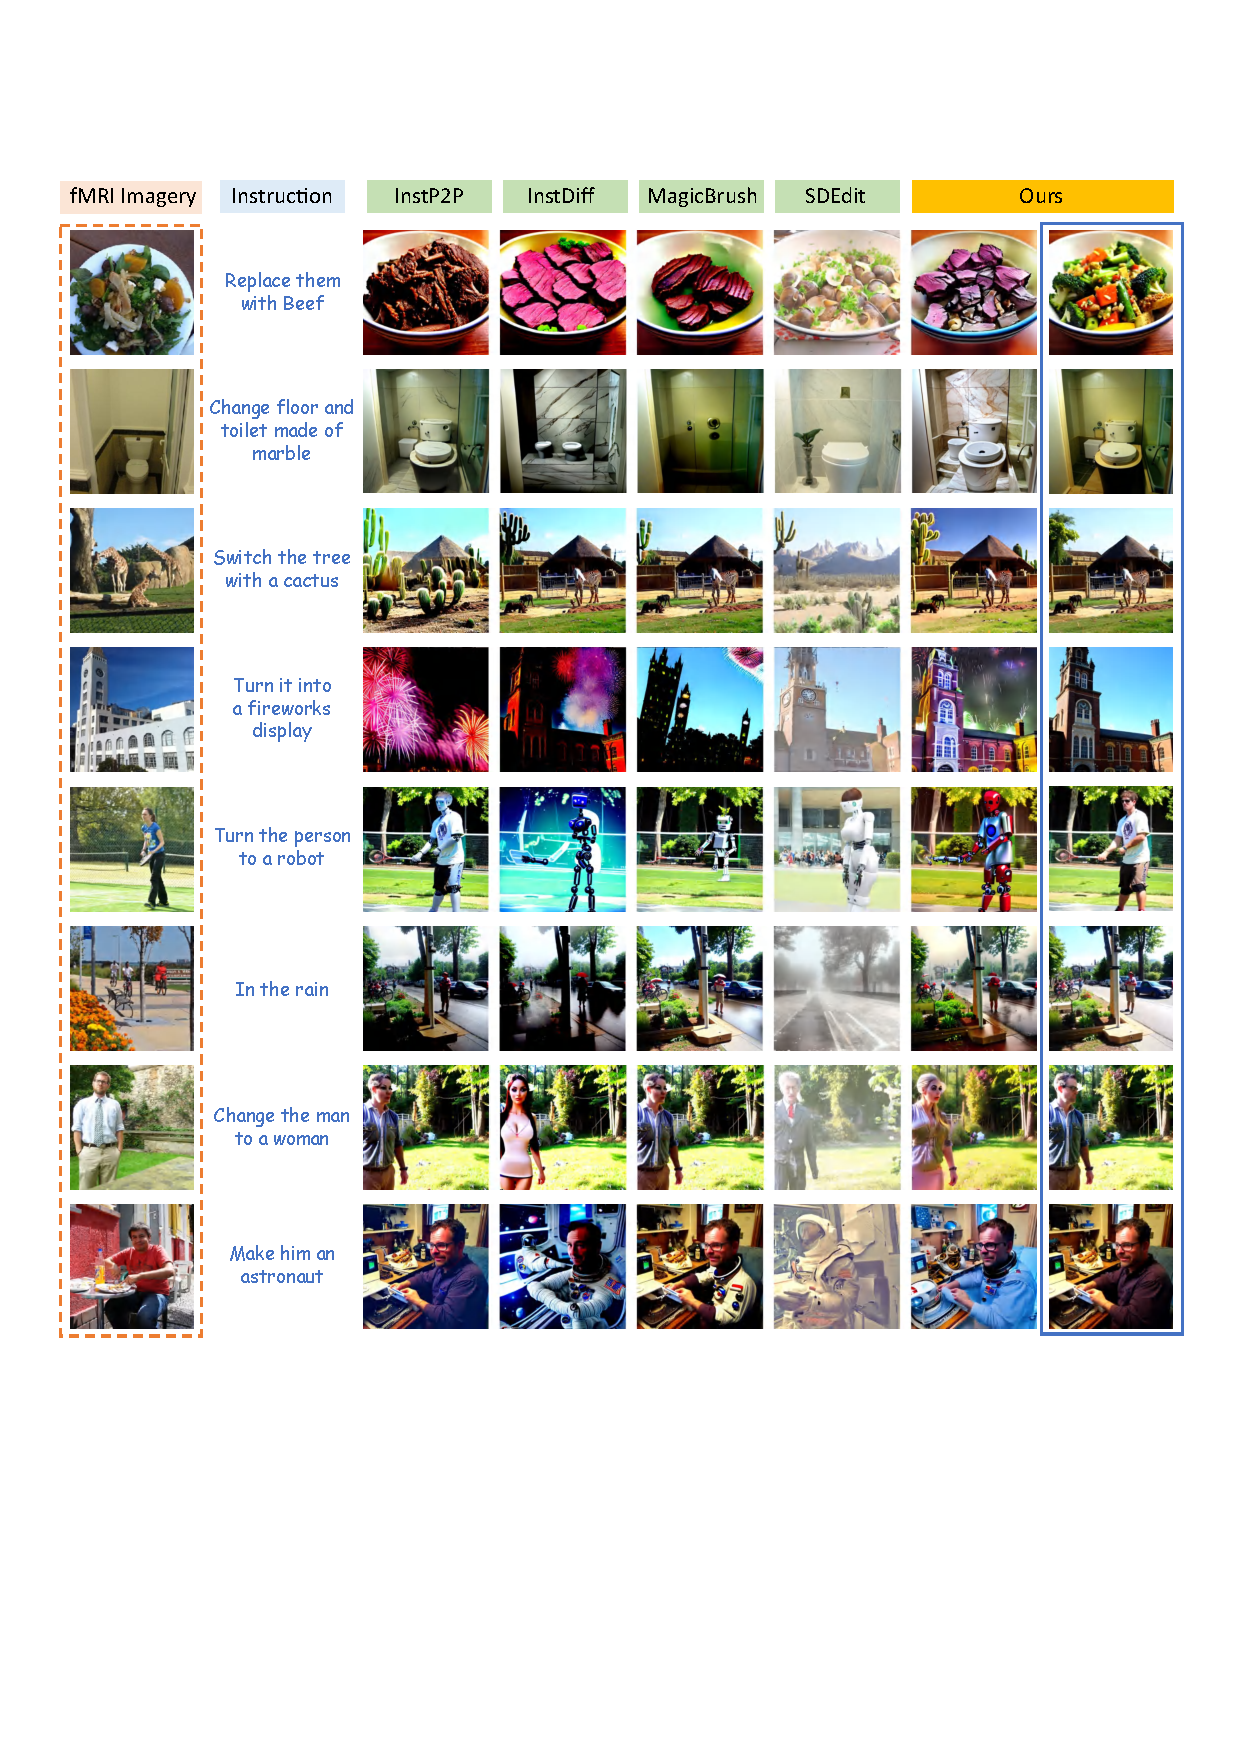
\includegraphics[width=\linewidth]{figs/qual1.pdf}
%   \caption{\textbf{Qualitative Comparison.} In the first column list the visual stimulus of fMRI signal while the last column demonstrates input images used by other approaches. InstP2P~\cite{brooks2023instructpix2pix} struggles on capturing instruction intention (see last 4 rows). InstDiff~\cite{geng2023instructdiffusion} and MagicBrush~\cite{zhang2024magicbrush} tends to over-edit irrelevant regions (see toilet). SDEdit~\cite{meng2021sdedit} suffers from inferior image quality. Our method well balances the content preservation and instruction conformation.
%   }
  \caption{\textbf{定性比较。} 第一列列出了 fMRI 信号的视觉刺激，而最后一列展示了其他方法所使用的输入图像。InstP2P~\cite{brooks2023instructpix2pix} 难以捕捉指令意图（见最后 4 行）。InstDiff~\cite{geng2023instructdiffusion} 和 MagicBrush~\cite{zhang2024magicbrush} 倾向于过度编辑无关区域（见马桶示例）。SDEdit~\cite{meng2021sdedit} 则面临图像质量较低的问题。我们的方法在内容保留与遵循指令之间取得了良好的平衡。
  }
  \label{fig:qual}
\end{figure*}

% \textbf{Image Generation Paradigm.} Since there are no similar studies supporting the direct instruction of fMRI signals, we adapt state-of-the-art image manipulation methods to evaluate the instruction capability of our model.
\textbf{图像生成范式。} 由于目前没有支持直接对 fMRI 信号发出指令的类似研究，我们将最先进的图像操纵方法进行了适配，以评估我们模型的指令能力。
% Specifically, we first generate fMRI instructions using our approach. We then use the obtained intermediate reconstruction $Y^{Rec}$, along with the instruction text, as input to these methods for editing.
具体而言，我们首先使用我们的方法生成 fMRI 指令结果。然后，我们将获取的中间重建图像 $Y^{Rec}$ 与指令文本一起作为输入，提供给这些方法进行编辑。

% \paragraph{Evaluation Results.} We demonstrate the qualitative evaluation results in Figure~\ref{fig:qual}.
\paragraph{评估结果。} 我们在图~\ref{fig:qual} 中展示了定性评估结果。
% We observe that InstructPix2Pix~\cite{brooks2023instructpix2pix} tends to preserve its original content and struggles to follow instructions (see the last 4 rows).
我们观察到 InstructPix2Pix~\cite{brooks2023instructpix2pix} 倾向于保留原始内容，难以遵循指令（见最后 4 行）。
% In contrast, InstructDiffusion~\cite{geng2023instructdiffusion} and MagicBrush~\cite{zhang2024magicbrush} are capable of better following instructions, but often change irrelevant attributes (e.g., the object shape such as the toilet and robot, or the background).
相比之下，InstructDiffusion~\cite{geng2023instructdiffusion} 和 MagicBrush~\cite{zhang2024magicbrush} 能够更好地遵循指令，但常常改变无关的属性（例如，诸如马桶和机器人等物体的形状，或背景）。
% For SDEdit~\cite{meng2021sdedit}, it also faces challenges in preserving unrelated regions and suffers from inferior image quality.
对于 SDEdit~\cite{meng2021sdedit}，它在保留无关区域方面同样面临挑战，并且生成的图像质量较差。
% In contrast, our approach strikes a balance between content preservation and instruction conformation (See the pose of the woman and the cactus shape), which we speculate is attributed to the dual-stream architecture where intermediate features are able to influence instruction progress constantly.
相反，我们的方法在内容保留与遵循指令之间取得了平衡（请见女人的姿势和仙人掌的形状），我们推测这归功于双流架构，其中中间特征能够持续地影响指令进度。
% It is worth noting that these approaches not only rely on our intermediate reconstruction results but also require tedious sequential operations. In contrast, our proposed framework enables direct fMRI signal instruction, streamlining the process.
值得注意的是，这些方法不仅依赖于我们的中间重建结果，还需要繁琐的串行操作。相比之下，我们提出的框架实现了直接对 fMRI 信号进行指令操作，从而精简了整个流程。

% \subsection{Additional Results}
\subsection{附加结果}

\begin{figure*}[t!]
  \centering
  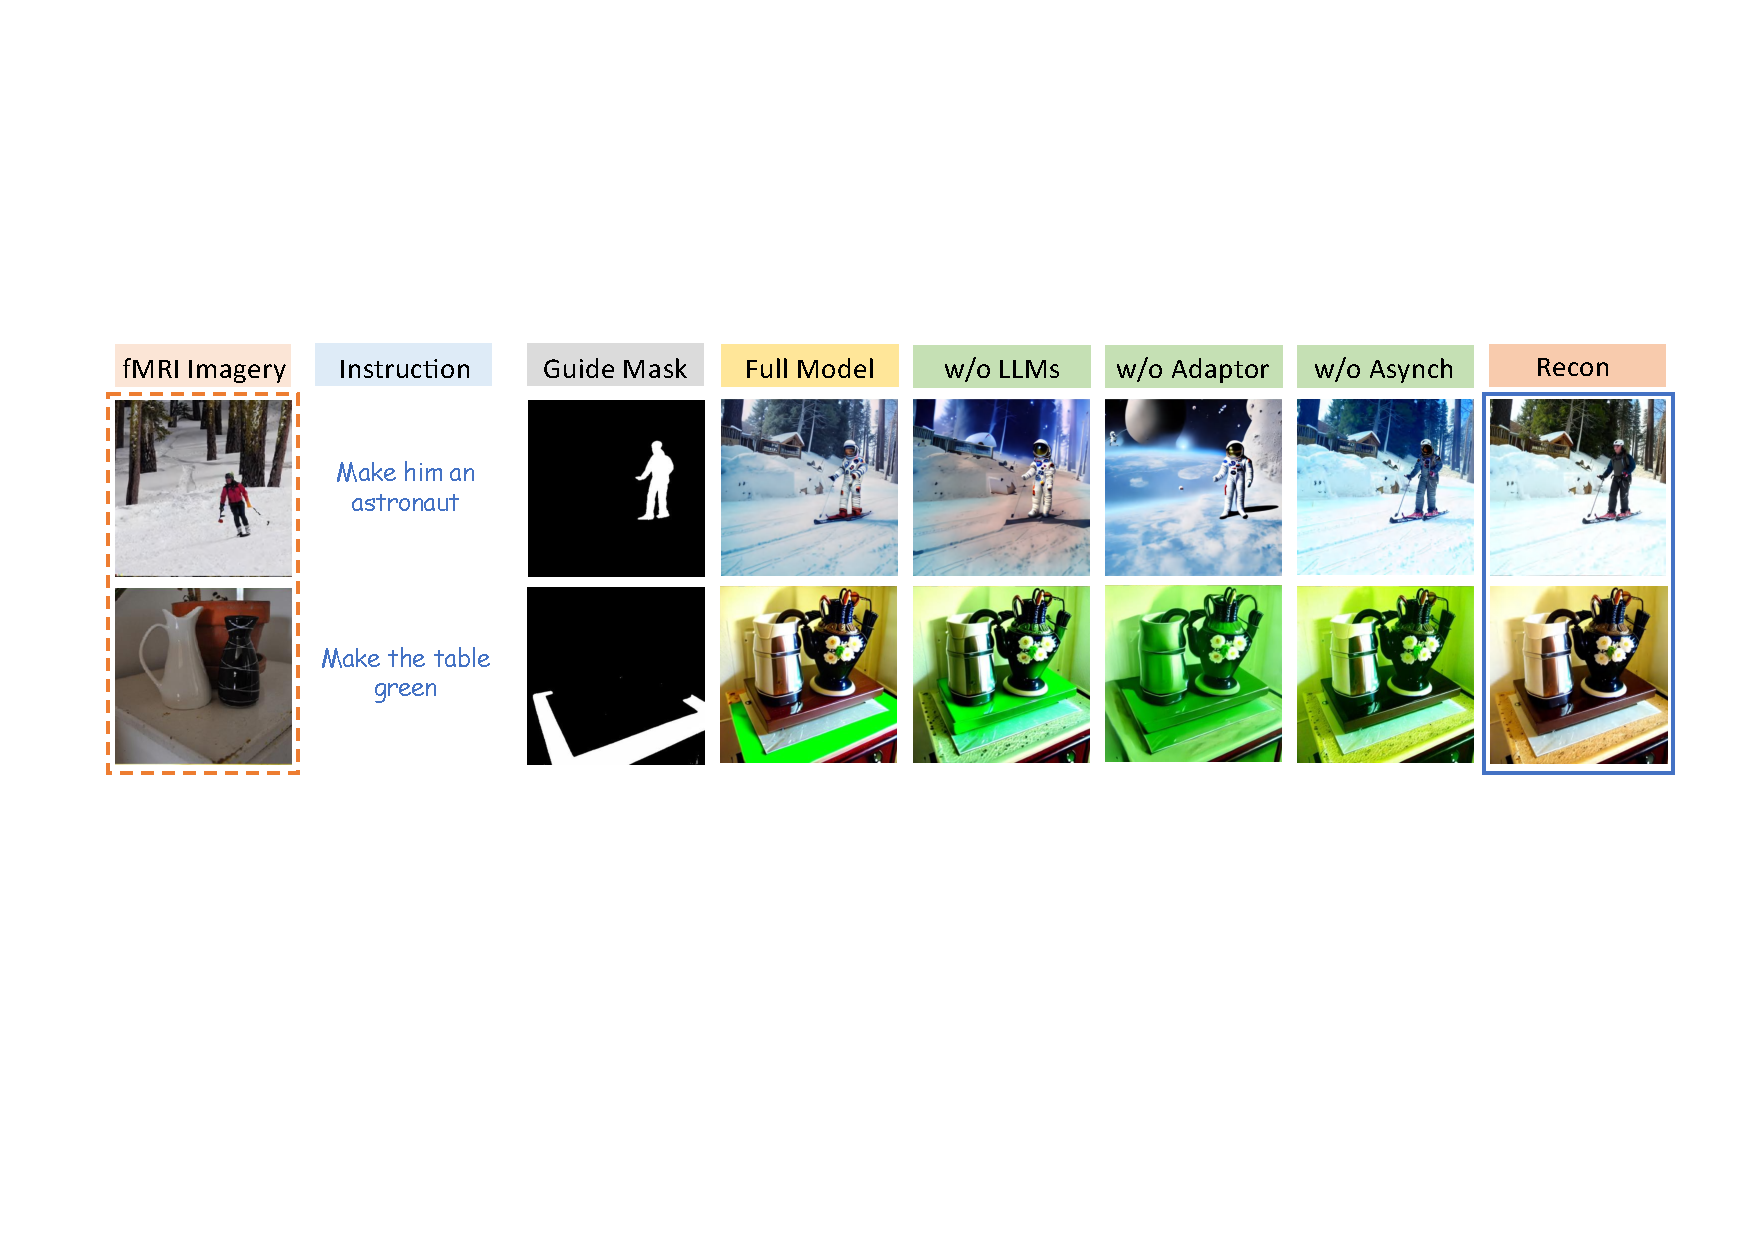
\includegraphics[width=1.0\linewidth]{figs/ablation1.pdf}
%   \caption{\textbf{Ablation Study.} Without feature injection from adaptor, the model struggles on balancing content preservation and instruction conformation. Removing asynchronous strategy brings difficulty on instruction conformation. Through the incorporation of LLMs guided region, our framework is able to precisely operate on relevant spatial locations (see the snow background and table region).
%   }
  \caption{\textbf{消融实验。} 如果没有来自适配器的特征注入，模型在平衡内容保留与遵循指令方面会面临困难。移除异步策略会给遵循指令带来难度。通过引入 LLM 引导的区域，我们的框架能够精确地在相关的空间位置上进行操作（见雪景背景和桌子区域的示例）。
  }
  \label{fig:ablation}
\end{figure*}

% \paragraph{Ablation Study.} We conducted ablation studies focusing on three important aspects of our method: the asynchronous diffusion strategy, the injection of adaptor features, and the use of LLM-guided region-aware attention.
\paragraph{消融实验。} 我们重点针对本方法的三个重要方面进行了消融实验：异步扩散策略、适配器特征的注入以及 LLM 引导的区域感知注意力的使用。
% The experiments were carried out by (1) removing the asynchronous paradigm, (2) eliminating adaptor feature injection, and (3) excluding the LLMs agent. The numerical results are shown in Table~\ref{table:ablation}, and the visualization results are presented in Fig.~\ref{fig:ablation}.
实验通过以下方式进行：(1) 移除异步范式，(2) 取消适配器特征注入，(3) 排除 LLM 代理。数值结果见表~\ref{table:ablation}，可视化结果展示在图~\ref{fig:ablation} 中。
% Eliminating the asynchronous strategy makes it difficult for the instruction flow to comprehend aligned visual content, resulting in inferior performance.
消除异步策略使得指令流难以理解对齐的视觉内容，导致性能下降。
% When adaptor feature injection is removed, the instruction flow lacks sufficient visual information to identify instruction-relevant regions. Consequently, the instruction results deviate from the interpreted visual contents of the first stream, leading to poor performance in terms of both CLIP and Dino image similarity.
当移除适配器特征注入时，指令流缺乏充足的视觉信息来识别与指令相关的区域。因此，指令结果偏离了第一流解释出的视觉内容，导致 CLIP 和 Dino 图像相似度的表现都不佳。
% Without LLMs, the model struggles to perform precise operations within the intended spatial regions.
如果没有 LLM，模型难以在预期的空间区域内执行精确操作。
% The full model effectively strikes a balance between identity preservation and instruction conformation, achieving visually pleasant results.
完整模型有效地在保持身份特征与遵循指令之间取得了平衡，实现了视觉上令人愉悦的结果。

% \paragraph{Multi-Modal Instruction.}
\paragraph{多模态指令。}
\begin{figure*}[t!]
  \centering
  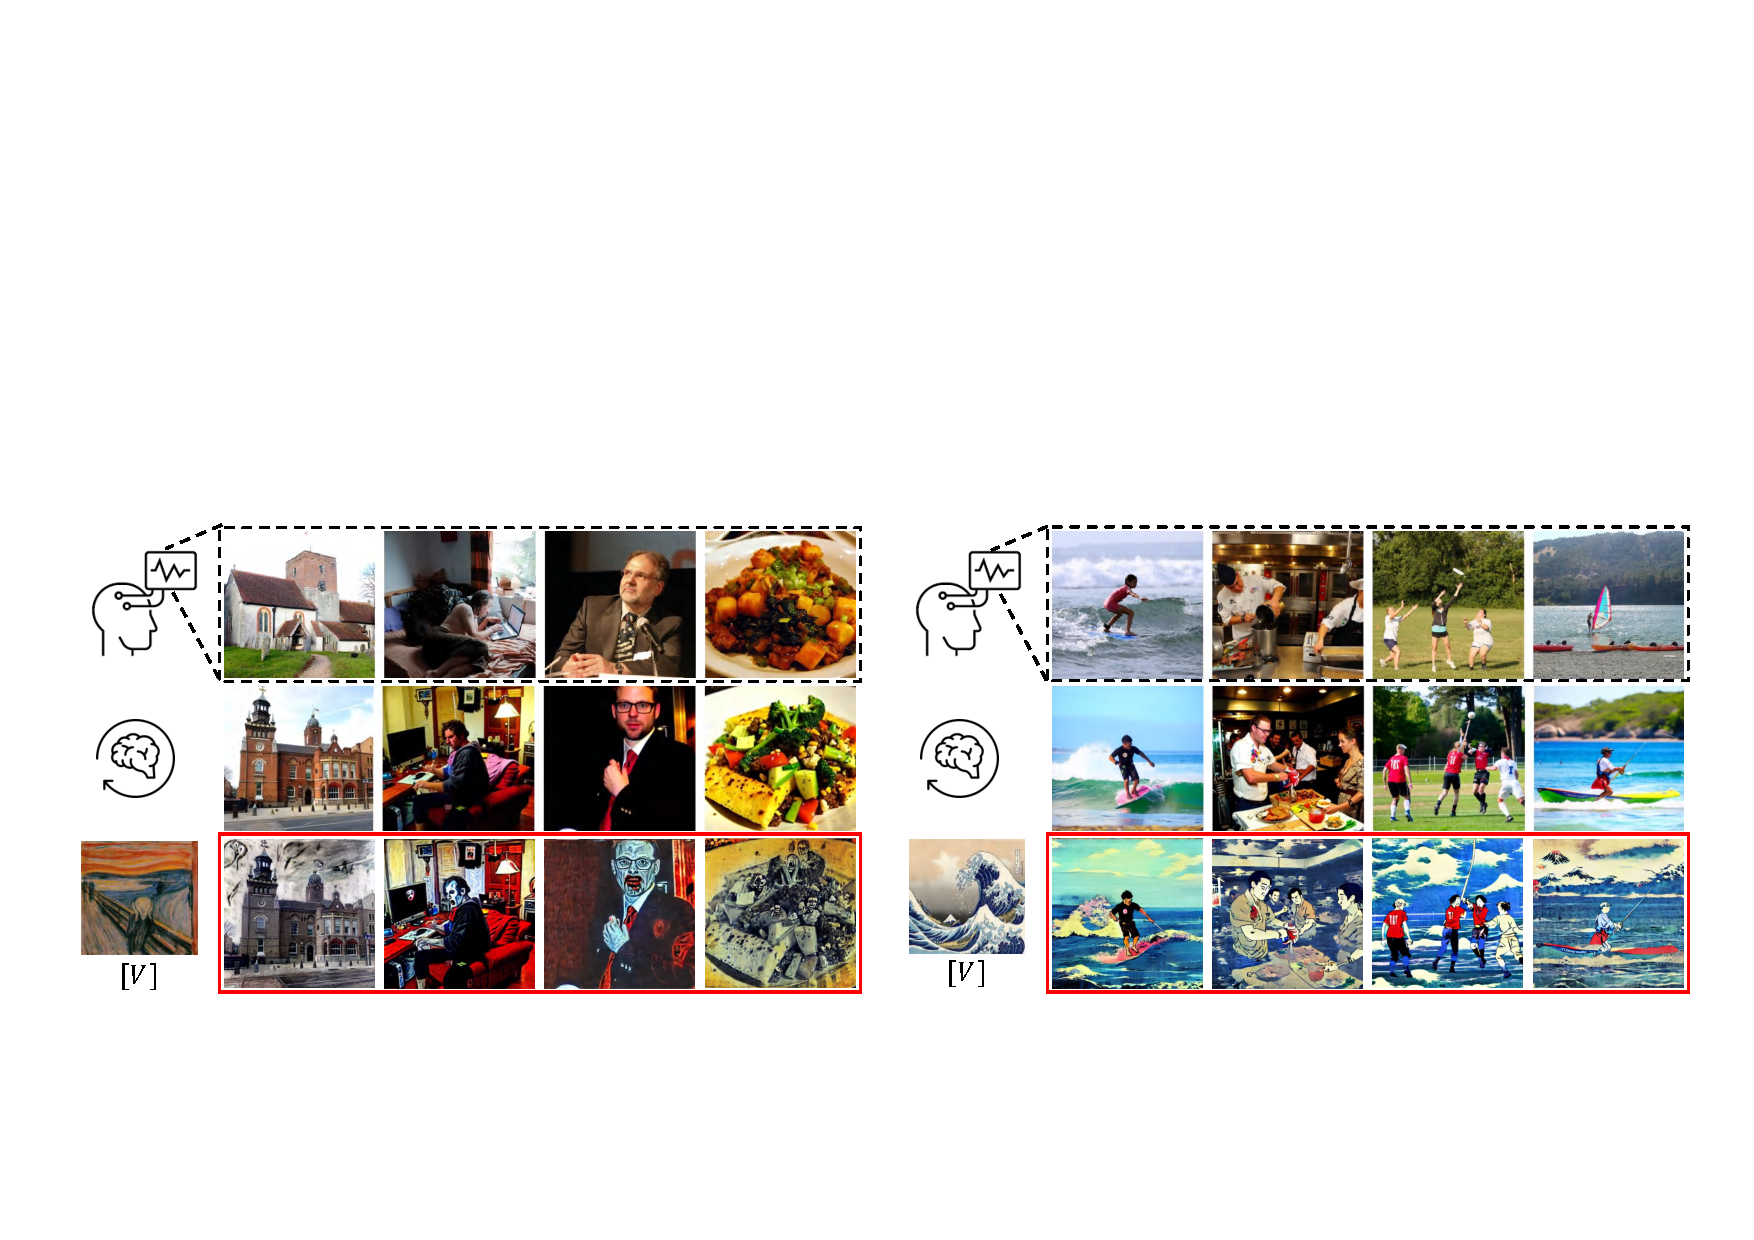
\includegraphics[width=1.0\linewidth]{figs/style.pdf}
%   \caption{\textbf{Demonstration Results of Multi-Modal Instruction.} First row list the visual stimulus while second row depict our intermediate reconstructions. The manipulation results via \emph{In the [V] style} are shown within red boxes of the last row.}
  \caption{\textbf{多模态指令演示结果。} 第一行展示了视觉刺激，第二行描绘了我们的中间重建结果。基于“\emph{以 [V] 风格（In the [V] style）}”的操纵结果显示在最后一行的红框内。}
  \label{fig:style}
\end{figure*}
% Here we showcase the ability of our model to handle multi-modal instruction and achieve style manipulation. With minimal effort, our model can be extended to support visual instruction.
在此，我们展示了模型处理多模态指令并实现风格操纵的能力。只需极少量的修改，我们的模型即可扩展为支持视觉指令。
% Specifically, we modify the instruction description to ``In the [V] style'' where the style ``[V]'' can be obtained using image inversion approaches~\cite{ruiz2023dreambooth,mokady2023null}. It is evident that our approach effectively captures the style of the reference image and applies it to the target.
具体来说，我们将指令描述修改为“以 [V] 风格”，其中风格“[V]”可以使用图像反演方法~\cite{ruiz2023dreambooth,mokady2023null}获得。显而易见，我们的方法有效地捕捉了参考图像的风格并将其应用于目标。
% \section{Conclusion}
\section{结论}

% In this paper, we propose \textbf{\model{}}, a framework that enables users to effectively interact with human "dreams" and influence final presentations.
在本文中，我们提出了 \textbf{\model{}}，这是一个能够让用户有效地与人类“梦境”进行交互并影响其最终呈现结果的框架。
% Our framework offers several appealing properties:
我们的框架具有以下几个吸引人的特性：
% 1) We \emph{pioneer a novel interaction paradigm with the human brain} by introducing a prototype that directly instructs fMRI signals via natural language descriptions, opening up exciting possibilities for future applications.
1) 我们\emph{开创了一种与人类大脑交互的新型范式}，通过引入一个原型系统，利用自然语言描述直接对 fMRI 信号发出指令，为未来的应用开辟了激动人心的可能性。
% 2) Our model's capability can be further enhanced using techniques that consider temporal and spatial perspectives, thereby improving the fidelity and precision of instructions.
2) 通过引入考虑时空视角的各项技术，我们可以进一步增强模型的能力，从而提高指令的保真度与精确度。
% 3) With minimal effort, our system can seamlessly extend to support multi-modal instructions.
3) 我们的系统只需极少量的改动，即可无缝扩展以支持多模态指令。

% \paragraph{Limitations and Future Work.} 1) In this work, we consider the obtained biological brain signals from visual stimuli as representations of human ``thoughts''. However, in real-world applications, the situation is more complex. ``Dreams,'' for instance, might originate from internal brain activity rather than external stimuli. 2) Our model struggles with instructions involving the addition of small objects. 3) For the LLM-enhanced region-aware instructions, an extra forward process is required to first extract the instruction-relevant regions from the intermediate reconstructions. 4) Future work will explore other types of ``dreams,'' such as audio and text, and more complex interaction strategies, such as multi-turn conversations.
\paragraph{局限性与未来工作。} 1) 在本研究中，我们将从视觉刺激中获取的生物脑信号视为人类“思想”的表征。然而在实际应用中，情况往往更加复杂。例如，“梦境”可能源自内部的大脑活动，而非外部刺激。2) 我们的模型在处理涉及添加细小对象的指令时存在困难。3) 对于基于大语言模型（LLM）增强的区域感知指令，需要额外的正向计算过程，才能从中间重建结果中提取出与指令相关的区域。4) 未来的工作将探索其他类型的“梦境”（如音频和文本），以及更复杂的交互策略（如多轮对话）。

% \paragraph{Ethical Issues.} As the title suggests, this model can be potentially exploited for malicious purposes such as mis-interpreting thoughts within human brain. We are committed to limiting the usage of our model strictly to research purposes.
\paragraph{伦理问题。} 正如标题所暗示的那样，该模型可能会被恶意利用，例如误解人类大脑中的真实想法。我们承诺严格限制我们模型的使用范围，确保其仅被用于研究目的。
% \section{Declarations}
\section{声明}

% \paragraph{Availability of Data and Material.}
\paragraph{数据及材料的可用性。}
% Our model and the involved dataset will be publicly available. Meanwhile, we will also release the instruction construction pipeline. The used fMRI signal and instruction pairs will be released for the research community to further explore this task.
我们的模型和相关数据集将公开发布。同时，我们也将开源指令构建的流水线代码。此外，我们还将发布所使用的 fMRI 信号与指令对，以供研究社区进一步探索这一任务。

% \paragraph{Competing Interests.}
\paragraph{竞争利益。}
% All authors certify that they have no affiliation or involvement in any organization or entity with any financial or non-financial interest in the subject matter or materials discussed in this manuscript.
所有作者均在此声明，未隶属于任何组织或实体，也未参与任何涉及本文所讨论的主题或材料且存在财务或非财务利益关系的组织或实体。

% \paragraph{Authors' Contributions.}
\paragraph{作者贡献。}
% Yasheng Sun coordinated the teamwork and proposed the overall method. Bohan Li trained the fMRI-to-Image module and conducted comparison results.
孙亚胜（Yasheng Sun）协调了团队工作并提出了整体方法。李博涵（Bohan Li）训练了 fMRI 到图像的生成模块并主导了对比实验结果的整理。
% Mingchen Zhuge initialized the idea of multi-modal learning with human brain activity signals and drafted the current version of the abstract and introduction. Prof. Fan manage the whole project. Prof. Fan, Prof. Salaman, Prof. Fahad, and Prof. Koike had insightful discussions and provided help polishing the manuscript.
诸葛鸣晨（Mingchen Zhuge）提出了结合人类大脑活动信号进行多模态学习的初步构想，并起草了当前版本的摘要与引言。范教授（Prof. Fan）管理了整个项目。范教授、Salaman 教授、Fahad 教授以及小池（Koike）教授参与了深刻的讨论，并在论文的润色方面提供了帮助。
% All authors read and approved the final manuscript.
所有作者均已阅读并同意最终定稿。

% \paragraph{Acknowledgements.}
\paragraph{致谢。}
% The authors express their gratitude to the anonymous reviewers and the editor, whose valuable feedback greatly improved the quality of this manuscript.
作者在此对匿名审稿人和编辑表示由衷的感谢，他们宝贵的反馈意见极大地提升了本稿件的质量。

\bibliographystyle{unsrt}
\bibliography{egbib}


\newpage
\clearpage
\appendix
\appendixpage

\section{Implementation Details}
\paragraph{Optimization Objective.} 
In addition to the typical MSE Loss~\cite{ho2020denoising} used in the Latent Diffusion Model (LDM), we also incorporate StyleCLIP~\cite{patashnik2021styleclip} loss to guide the model toward the correct manipulation direction.  Formally,

\begin{equation}
\begin{aligned}
    \mathcal{L}_{style} &= 1 - \\
    \mathcal{D}(
    \textbf{F}_{vis}(\hat{Y}^{edit}) &- \textbf{F}_{vis}(Y), 
    \textbf{F}_{text}(T^{edit}) - \textbf{F}_{text}(T)),
\end{aligned}
\end{equation}

where $\mathcal{D}$ indicates the cosine similarity between two vectors. 
$Y$ and $T$ represent the original visual stimuli and its corresponding text, while the $\hat{Y}^{edit}$ and $T^{edit}$ are the synthesized result produced by our network and its corresponding ground truth caption, respectively. $\hat{Y}^{edit}$ can be estimated at each time step as follows:
\begin{equation}
\label{eq:decode_z}
    \hat{\textbf{z}}_0^e = (\textbf{z}_t^e - \sqrt{1-\overline{\alpha}_t} \bm{\epsilon}_{\theta} (\textbf{z}_t^e)) / \sqrt{\overline{\alpha}}_t,
\end{equation}
where the $\overline{\alpha}_t := \prod_{s=1}^t \alpha_s$. 
$\hat{Y}^{edit}$ can be decoded from $\hat{\textbf{z}}_0^e$.
The functions $\textbf{F}_{vis}$ and $\textbf{F}_{text}$ represent the CLIP backbone used to extract the visual and text features, respectively.
Such formulation ensures that the editing direction of the synthesized image aligns closely with the text direction in CLIP space.
The overall loss function, which combines the style direction loss with the foundational LDM loss, is mathematically represented as:
\begin{equation}
\mathcal{L}=\mathcal{L}_{simple}+\sqrt{\bar{\alpha}_t} \mathcal{L}_{style},
\end{equation}
where $\sqrt{\bar{\alpha}_t}$ is leveraged to emphasize the supervision with lower noise input (i.e., smaller time-step) and reduce the impact with higher noise (i.e., larger time-step).



\paragraph{Inference Paradigm.} Given a target fMRI signal $X$, our goal is to interact with it through the instruction $I$. The primary objective is to manipulate the visual content within the human brain toward the desired direction, resulting in $Y^{edit}$. During inference, we first use $\bm{g}_\theta(\textbf{z}^r_t, X, t)$ to perform $K$ diffusion steps for basic feature formation from $X$. Building on this, the dual-stream diffusion model $\bm{\epsilon}_\theta(\textbf{z}^r_t, \textbf{z}^e_t, I, X, t)$ progressively guides the fMRI signal.
After the diffusion process is complete, the latent code $\textbf{z}_0^e$ is transformed back to $Y^{edit}$ following Equation~\ref{eq:decode_z}. The detailed inference process is depicted in Algorithm~\ref{alg:test}.

\begin{algorithm*}[!ht]
  \caption{Inference of the asynchronous dual-stream diffusion model $\bm{\epsilon}_{\theta}$}
  \label{alg:sampling}
  \label{alg:test}
  \small
  \begin{algorithmic}[1]
    \vspace{.04in}
    \State $  \textbf{z}_T^e \sim \mathcal{N}(\mathbf{0}, \mathbf{I}), $ $  \textbf{z}_T^r \sim \mathcal{N}(\mathbf{0}, \mathbf{I})  $

    \For{$t=T, \dotsc, T-K+1$}
      \State $\textbf{z}^{nr} \sim \mathcal{N}(\mathbf{0}, \mathbf{I})$
      \State $\textbf{z}^r_{t-1} = \frac{1}{\sqrt{\alpha_t}}\left( \textbf{z}^r_{t} - \frac{1-\alpha_t}{\sqrt{1-\bar{\alpha}_t}} \bm{g}_\theta(\textbf{z}^r_{t}, X,t) \right) + \sigma_t \textbf{z}^{nr}$
    \EndFor

    \For{$t=T, \dotsc, K+1$}
      \State $\textbf{z}^{nr} \sim \mathcal{N}(\mathbf{0}, \mathbf{I})$ if $t > K+1$, else $\textbf{z}^{nr} = \mathbf{0}$
      \State $\textbf{z}^{ne} \sim \mathcal{N}(\mathbf{0}, \mathbf{I})$
      \State $\textbf{z}^r_{t\textcolor{red}{-K}-1} = \frac{1}{\sqrt{\alpha_{t\textcolor{red}{-K}}}}\left( \textbf{z}^r_{t\textcolor{red}{-K}} - \frac{1-\alpha_{t\textcolor{red}{-K}}}{\sqrt{1-\bar{\alpha}_{t\textcolor{red}{-K}}}} \bm{g}_\theta(\textbf{z}^r_{t\textcolor{red}{-K}}, X,t\textcolor{red}{-K}) \right) + \sigma_{t\textcolor{red}{-K}} \textbf{z}^{nr}$
      \State $\textbf{z}^e_{t-1} = \frac{1}{\sqrt{\alpha_t}}\left( \textbf{z}^e_{t} - \frac{1-\alpha_t}{\sqrt{1-\bar{\alpha}_t}} \bm{\epsilon}_\theta(\textbf{z}^r_{t\textcolor{red}{-K}}, \textbf{z}^e_{t}, I,X,t) \right) + \sigma_t \textbf{z}^{ne}$
    \EndFor

    \For{$t=K, \dotsc, 1$}
      \State $\textbf{z}^{ne} \sim \mathcal{N}(\mathbf{0}, \mathbf{I})$ if $t > 1$, else $\textbf{z}^{ne} = \mathbf{0}$
      \State $\textbf{z}^e_{t-1} = \frac{1}{\sqrt{\alpha_t}}\left( \textbf{z}^e_{t} - \frac{1-\alpha_t}{\sqrt{1-\bar{\alpha}_t}} \bm{\epsilon}_\theta(\textbf{z}^r_0, \textbf{z}^e_{t}, I,X,t) \right) + \sigma_t \textbf{z}^{ne}$

    \EndFor
    
    \State \textbf{return} $\textbf{z}^e_0$
    \vspace{.04in}
  \end{algorithmic}
\end{algorithm*}

\paragraph{Training Paradigm.}
During training, the denoising operation is performed asynchronously, with the instruction flow lagging behind by $K$ time steps. The detailed training process of our dual-stream diffusion framework is outlined in Algorithm~\ref{alg:training}.

\begin{algorithm*}[h]
  \caption{Training of the asynchronous dual-stream diffusion model $\bm{\epsilon}_{\theta}$}
  \label{alg:training}
  \small
  \begin{algorithmic}[1]
    \Repeat
      \State $(\textbf{z}_0^e, \textbf{z}_0^r, I, X) \sim q(\textbf{z}_0^e, \textbf{z}_0^r, I, X)$
      \State $\bm{\epsilon} \sim \mathcal{N}(\mathbf{0}, \mathbf{I}), \bm{\epsilon}^r \sim \mathcal{N}(\mathbf{0}, \mathbf{I})$
      \State $t \sim \text{Uniform}({K+1,\ldots,T})$
      \State Take a gradient descent step on
      \State 
      $ \quad \nabla_\theta \left\| \bm{\epsilon} - \bm{\epsilon}_\theta(\sqrt{\bar{\alpha}_{t\textcolor{red}{-K}}} \textbf{z}_0^r+\sqrt{1-\bar{\alpha}_{t\textcolor{red}{-K}}} \bm{\epsilon}^r, 
      \sqrt{\bar{\alpha}_{t}} \textbf{z}_0^e+\sqrt{1-\bar{\alpha}_{t}} \bm{\epsilon}, I, X, t) \right\|$
    \Until{converged}
  \end{algorithmic}
\end{algorithm*}


\section{More Ablation Studies}
In this section, we provide a detailed quantitative analysis of the components involved in our method.
Firstly, we present both qualitative and quantitative results to illustrate the impact of varying asynchronous steps.
Next, we offer further insights into the design of the dual-stream architecture.
Finally, we include additional qualitative ablation results to demonstrate the effect of each part of our architecture.

\paragraph{Impact of Varied Asynchronous Steps.} To investigate the impact of delayed steps on model performance, we conduct experiments with varied time steps. Specifically, in our implementation, we adopt $T=50$ at inference for efficiency. Thus, we choose $K=0, 5, 15, 25, 35$, which are broadly distributed, to conduct the experiment. For the sake of comparison, we do not incorporate LLMs and manually fix the random seed for all settings. Table~\ref{table:ablate_time_steps} illustrates the impact of delayed time steps. We observe that overall performance improves as we increase the delayed time steps, but the improvement becomes marginal beyond $K=15$. This is likely because $K=15$ is sufficient for basic feature formation.


% Table 2%%%%%%%%%%%%%%%%%%%%%%%%%%%%%%%%%%%%%%%%%%%%%%%%%%%%%%%%%%%%
\begin{table*}[h] %\footnotesize
\setlength{\tabcolsep}{28pt}
\begin{center}  
\caption{\textbf{The impact of different delayed time steps on model performance.}}
% \vspace{-2pt}
\label{table:ablate_time_steps}
\begin{tabular}{lcccccccc}
\toprule
 % & \multicolumn{4}{c}{Low-Level}& \multicolumn{4}{c}{High-Level} \\
% \cmidrule(lr){2-5} \cmidrule(lr){6-9}
Delay Steps & 0 & 5 &  15 & 25 &
35 \\

\midrule  
\textbf{CLIP-I} & 0.636 & 0.638 & \textbf{0.642} & 0.642 & 0.641  \\
\textbf{Dino-I} & \textbf{0.307} & 0.307 & 0.295 & 0.295 & 0.293 \\
\textbf{CLIP-D} & 0.108 & 0.109 & \textbf{0.114} & 0.106 & 0.108 \\
% \hline
% \textbf{Mind-Sculpting}  & \textbf{0.327} & 0.315 & \textbf{0.951} & \textbf{0.978} & \textbf{0.939} \\
\bottomrule
\end{tabular}
\end{center}
% \vspace{-12pt}
\end{table*}
% Table 2%%%%%%%%%%%%%%%%%%%%%%%%%%%%%%%%%%%%%%%%%%%%%%%%%%%%%%%%%%%%



To further demonstrate the effect of the asynchronous strategy, we present the intermediate manipulation process in Fig.\ref{fig:async_demo}. We compare the synchronous strategy (set $K=0$ in the second row) with the asynchronous strategy (set $K=15$ in the third row). The individual intends to "Make it a unicorn" to manipulate brain activity. In the synchronous scenario, the model fails to capture the pertinent structure, i.e., the horse, for effective instruction (as indicated by the color of the horse within the red box). Without allowing basic feature formation in advance, the instruction model encounters difficulty in identifying the relevant structure. For additional visual results, readers can refer to Fig.\ref{fig:async_all_supp}.



\begin{figure*}[ht!]
  \centering
  % \vspace{-10pt}
  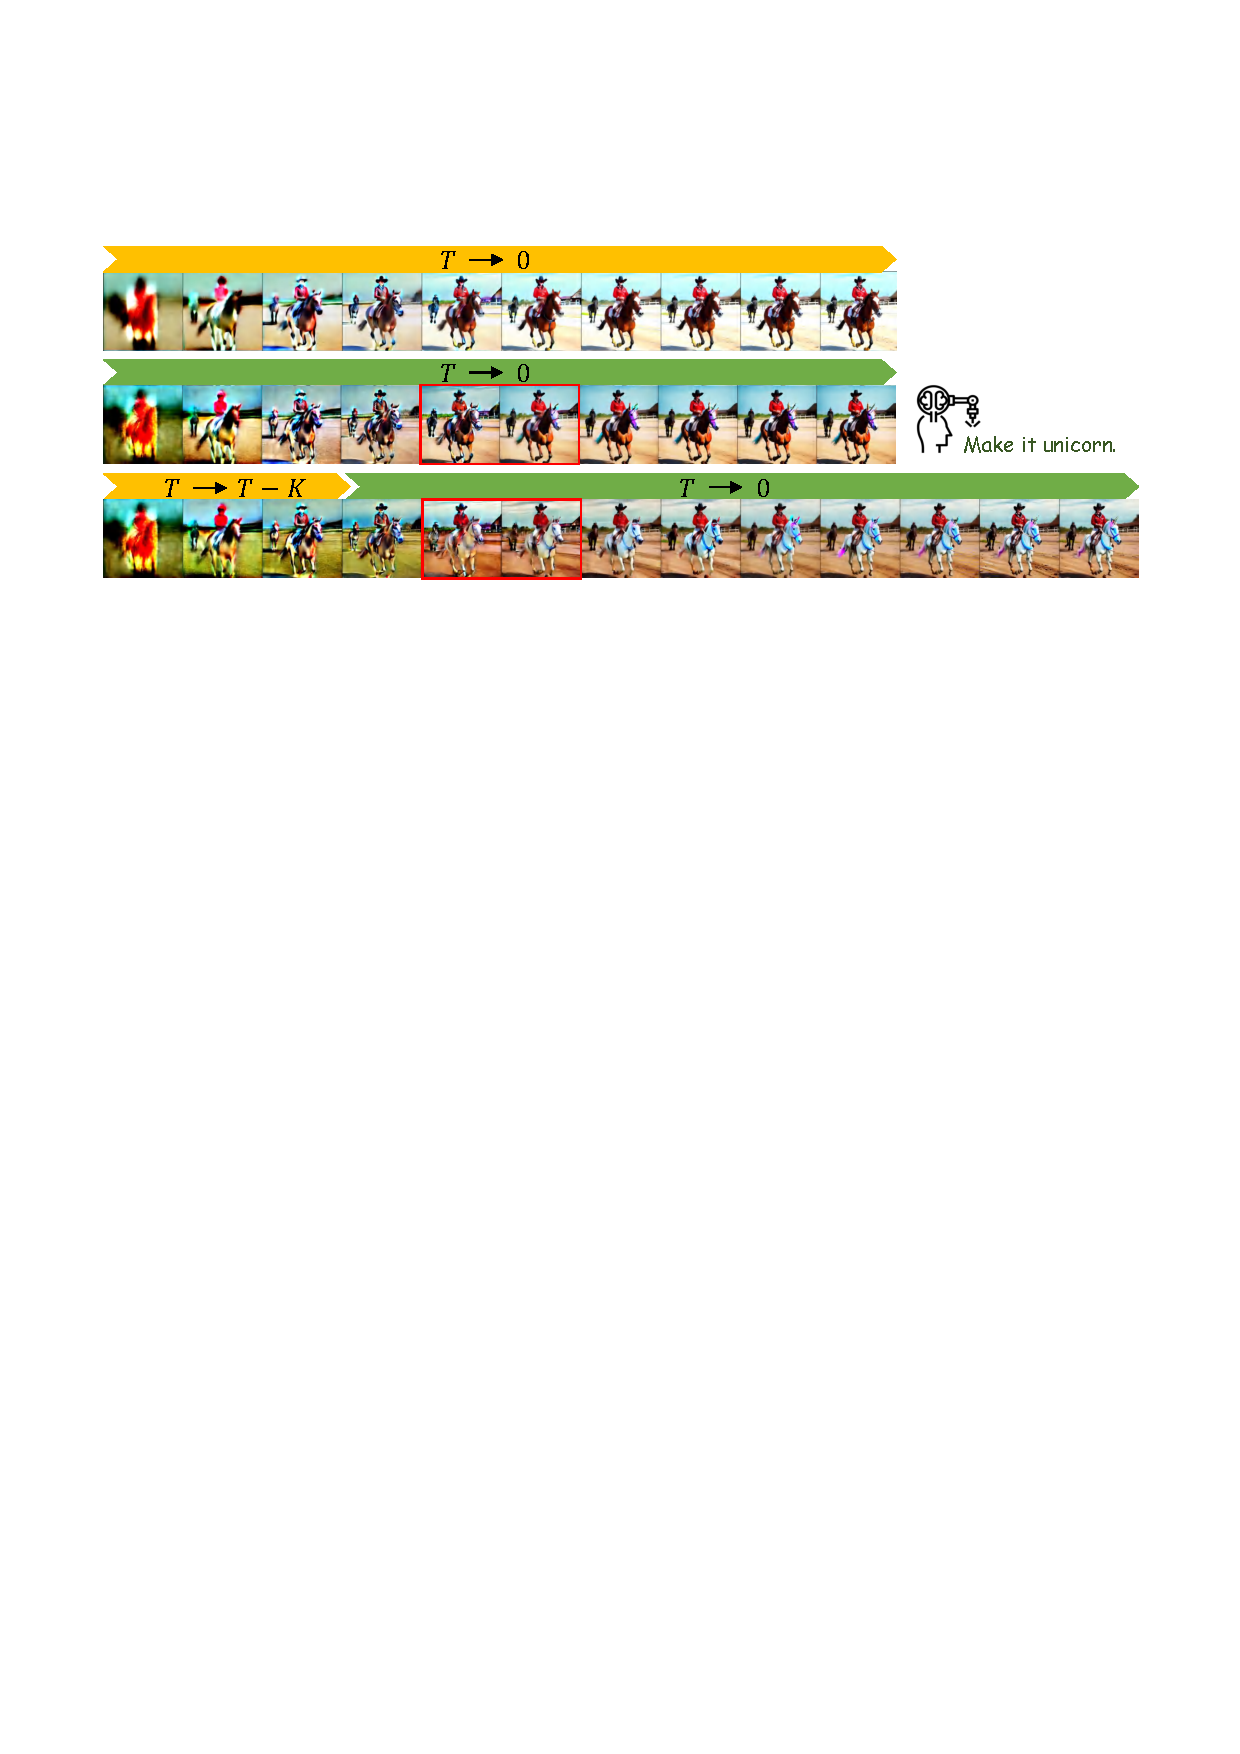
\includegraphics[width=1.0\linewidth]{figs/async_demo.pdf}
  \caption{The first row displays the intermediate reconstruction results, while the second and third rows showcase the instruction performance using synchronous and asynchronous paradigms, respectively. The orange progress bar indicates the reconstruction timeline, while the green progress bar represents the instruction timeline.}
  \label{fig:async_demo}
\end{figure*}


\begin{figure*}[ht!]
  \centering
  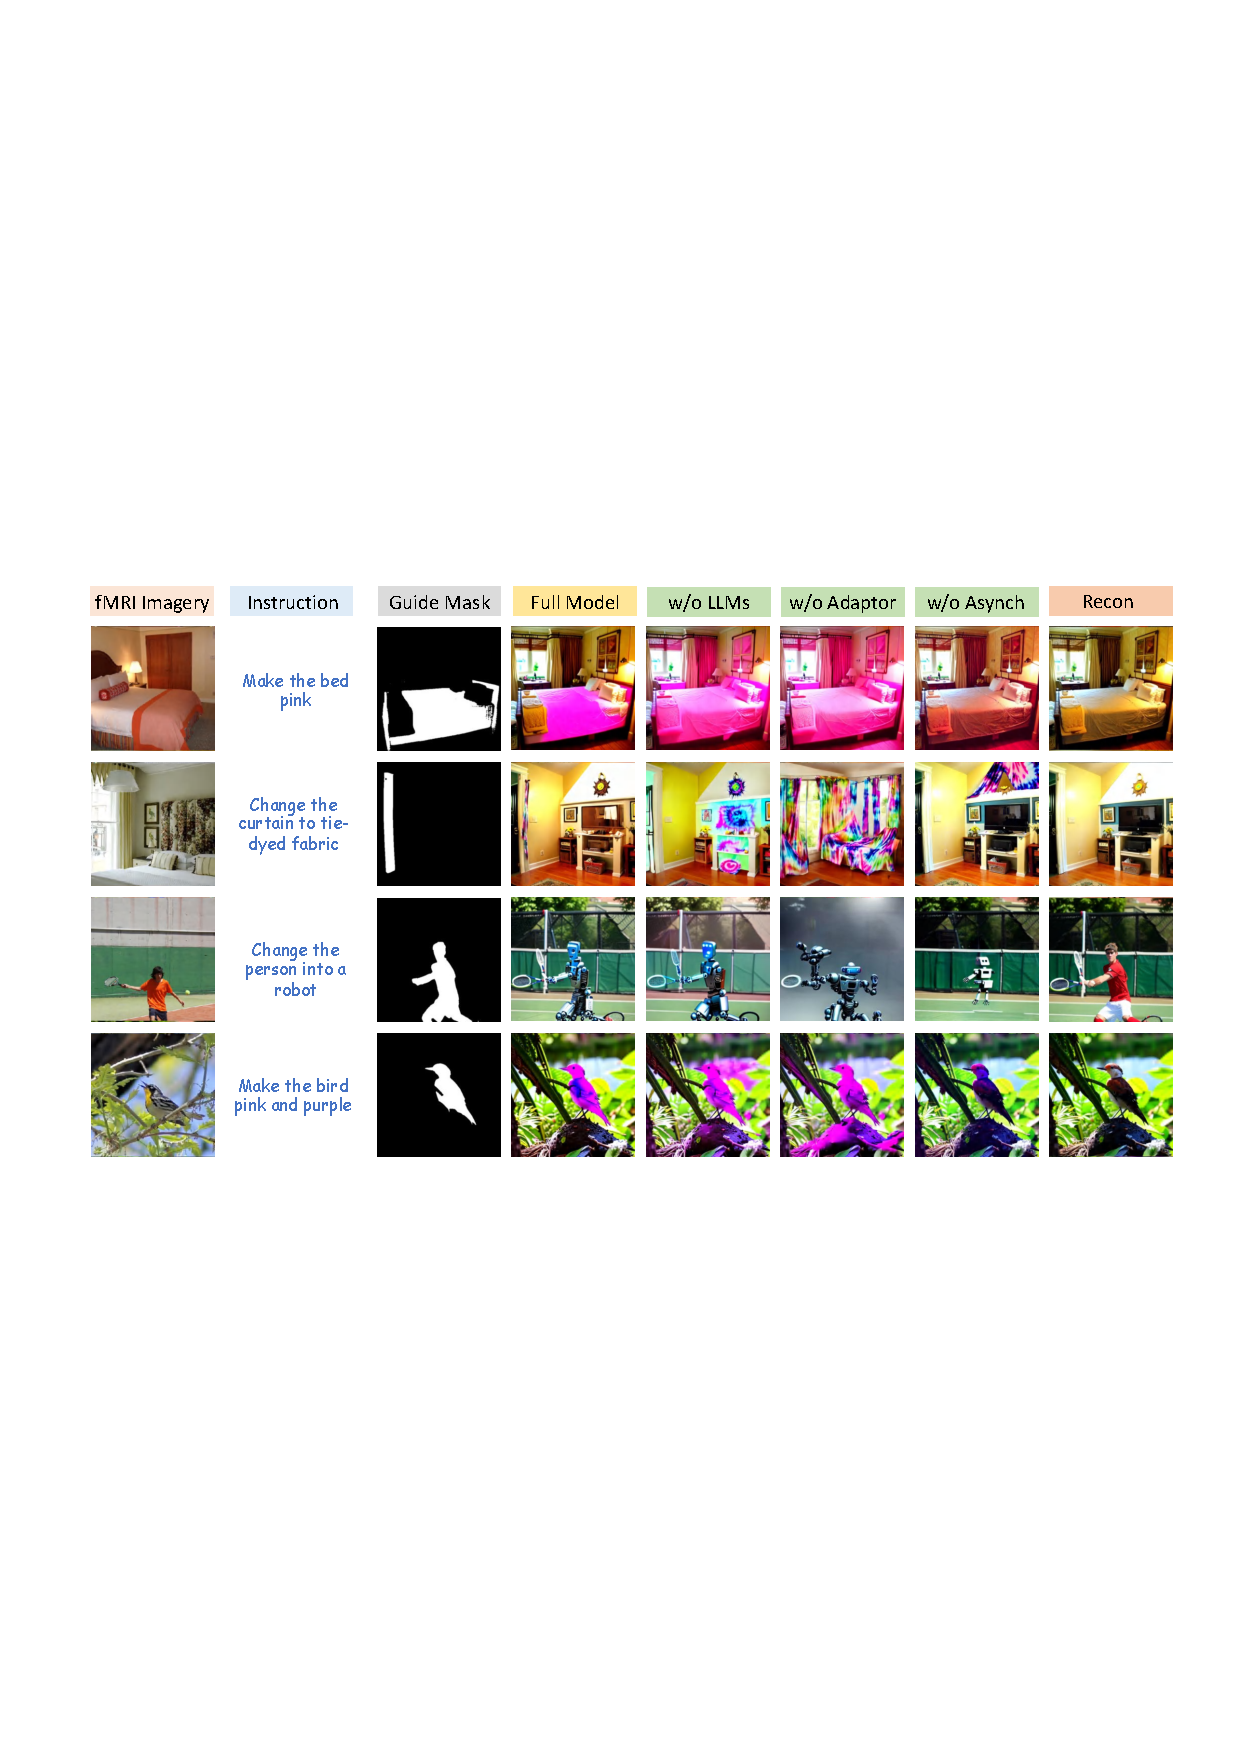
\includegraphics[width=1.0\textwidth]{figs/more_ablations.pdf} 
    % \vspace{-4pt}
  \caption{Without feature injection from adaptor, the model struggles on balancing content preservation and instruction conformation. Removing asynchronous strategy brings difficulty on instruction conformation. Through the incorporation of LLMs guided region, our framework is able to precisely operate on relevant spatial locations.}
  \label{fig:more_ablation}
  % \vspace{-5pt}
\end{figure*}


\paragraph{Impact of Injection Strategy.} The feature injection module acts as a connector, linking the instruction flow to the generation flow, ensuring seamless progressive bridging and effective instruction delivery. For the architecture design of our injection module, we explored both convolution-based structures~\cite{zhang2023adding} and transformer-based structures~\cite{hu2023animate}. Experiments demonstrate that the transformer-based architecture does not improve performance. We speculate this is because the convolution operation's advantage in maintaining spatial layout facilitates learning. Regarding the injection strategy, we empirically found that injection through ResBlock outperforms other blocks. Additionally, leveraging more advanced fusion techniques, such as transformers, does not enhance our performance.

\paragraph{More Qualitative Results.} We demonstrate additional visual results of our ablation study in Fig.~\ref{fig:more_ablation}. Eliminating the asynchronous strategy makes it difficult for the instruction flow to comprehend the aligned visual content, leading to inferior performance (see the bed and robot). Without the feature injection from the adaptor, the instruction flow lacks sufficient visual information to identify instruction-relevant regions (see the mis-edited curtain and bird). Without LLMs, the model struggles to perform precise operations within the intended spatial regions (see the bed and the bird). The full model effectively balances identity preservation and instruction conformation, achieving visually pleasing results.

\section{More fMRI Instruction Results}
In this section, we present additional visual instruction results. Although our approach is designed for language-guided instruction, it can readily extend to visual instruction with minimal effort.

\paragraph{Natural Language Instruction.}
We demonstrate more instruction results in Fig.~\ref{fig:supp_edit0} and Fig.~\ref{fig:supp_edit1}.
It can be seen that our approach is able to effectively interface with brain activity conforming to human instructions.

\paragraph{Style Manipulation.}
For style manipulation, we first invert the style reference image to a word embedding ${[V]}$ in the text latent space, following the common inversion strategy~\cite{ruiz2023dreambooth,mokady2023null}. We then use \emph{In the style of} $[V]$ as our new instruction. The results of this instruction are depicted in Fig.~\ref{fig:supp_style}. It can be seen that our approach effectively captures the style of the reference image and applies it to the target.


\begin{figure*}[ht!]
  \centering
  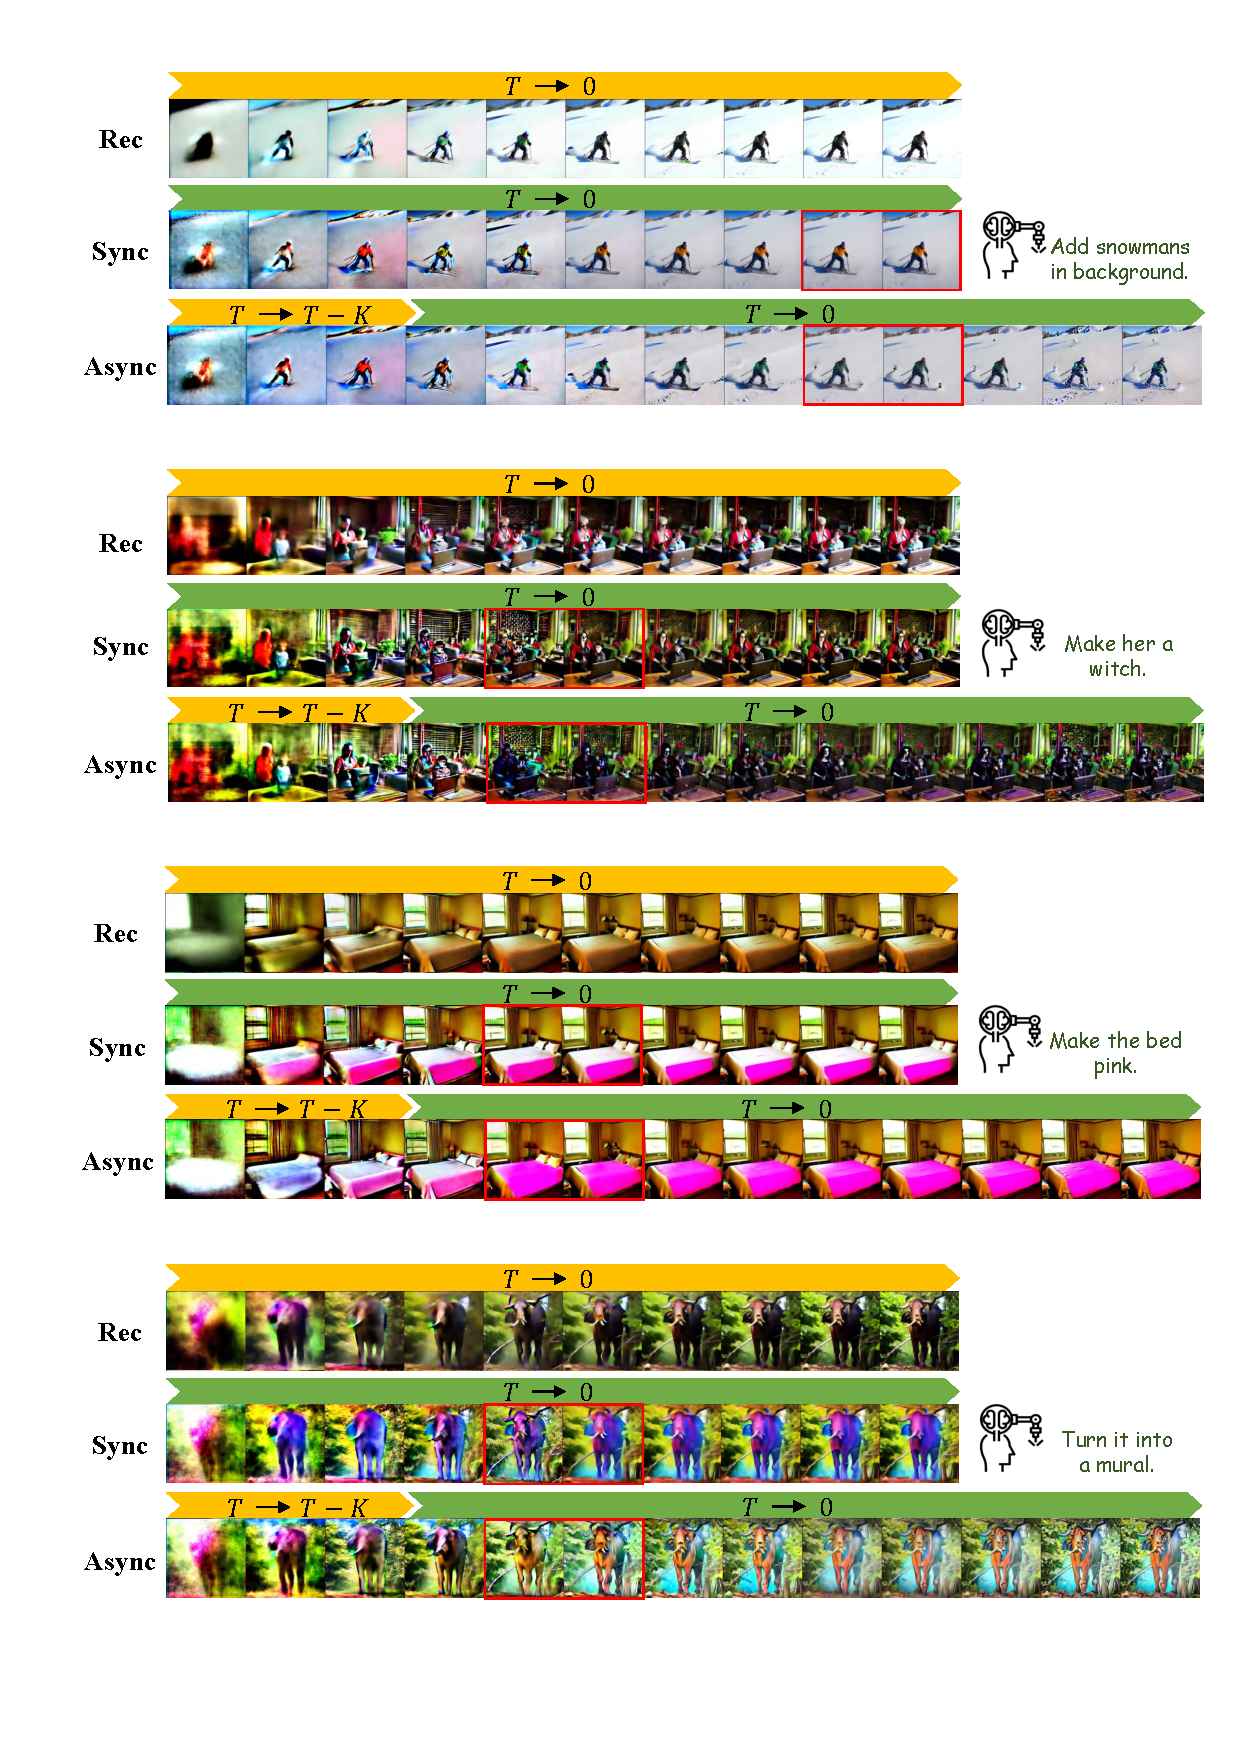
\includegraphics[width=1.0\textwidth]{figs/async_all_supp.pdf} 
    % \vspace{-4pt}
  \caption{The first row displays the intermediate reconstruction results, while the second and third rows showcase the instruction performance using synchronous and asynchronous paradigms, respectively. The orange progress bar indicates the reconstruction timeline, while the green progress bar represents the instruction timeline.}
  \label{fig:async_all_supp}
  % \vspace{30pt}
\end{figure*}



\begin{figure*}[ht!]
  \centering
  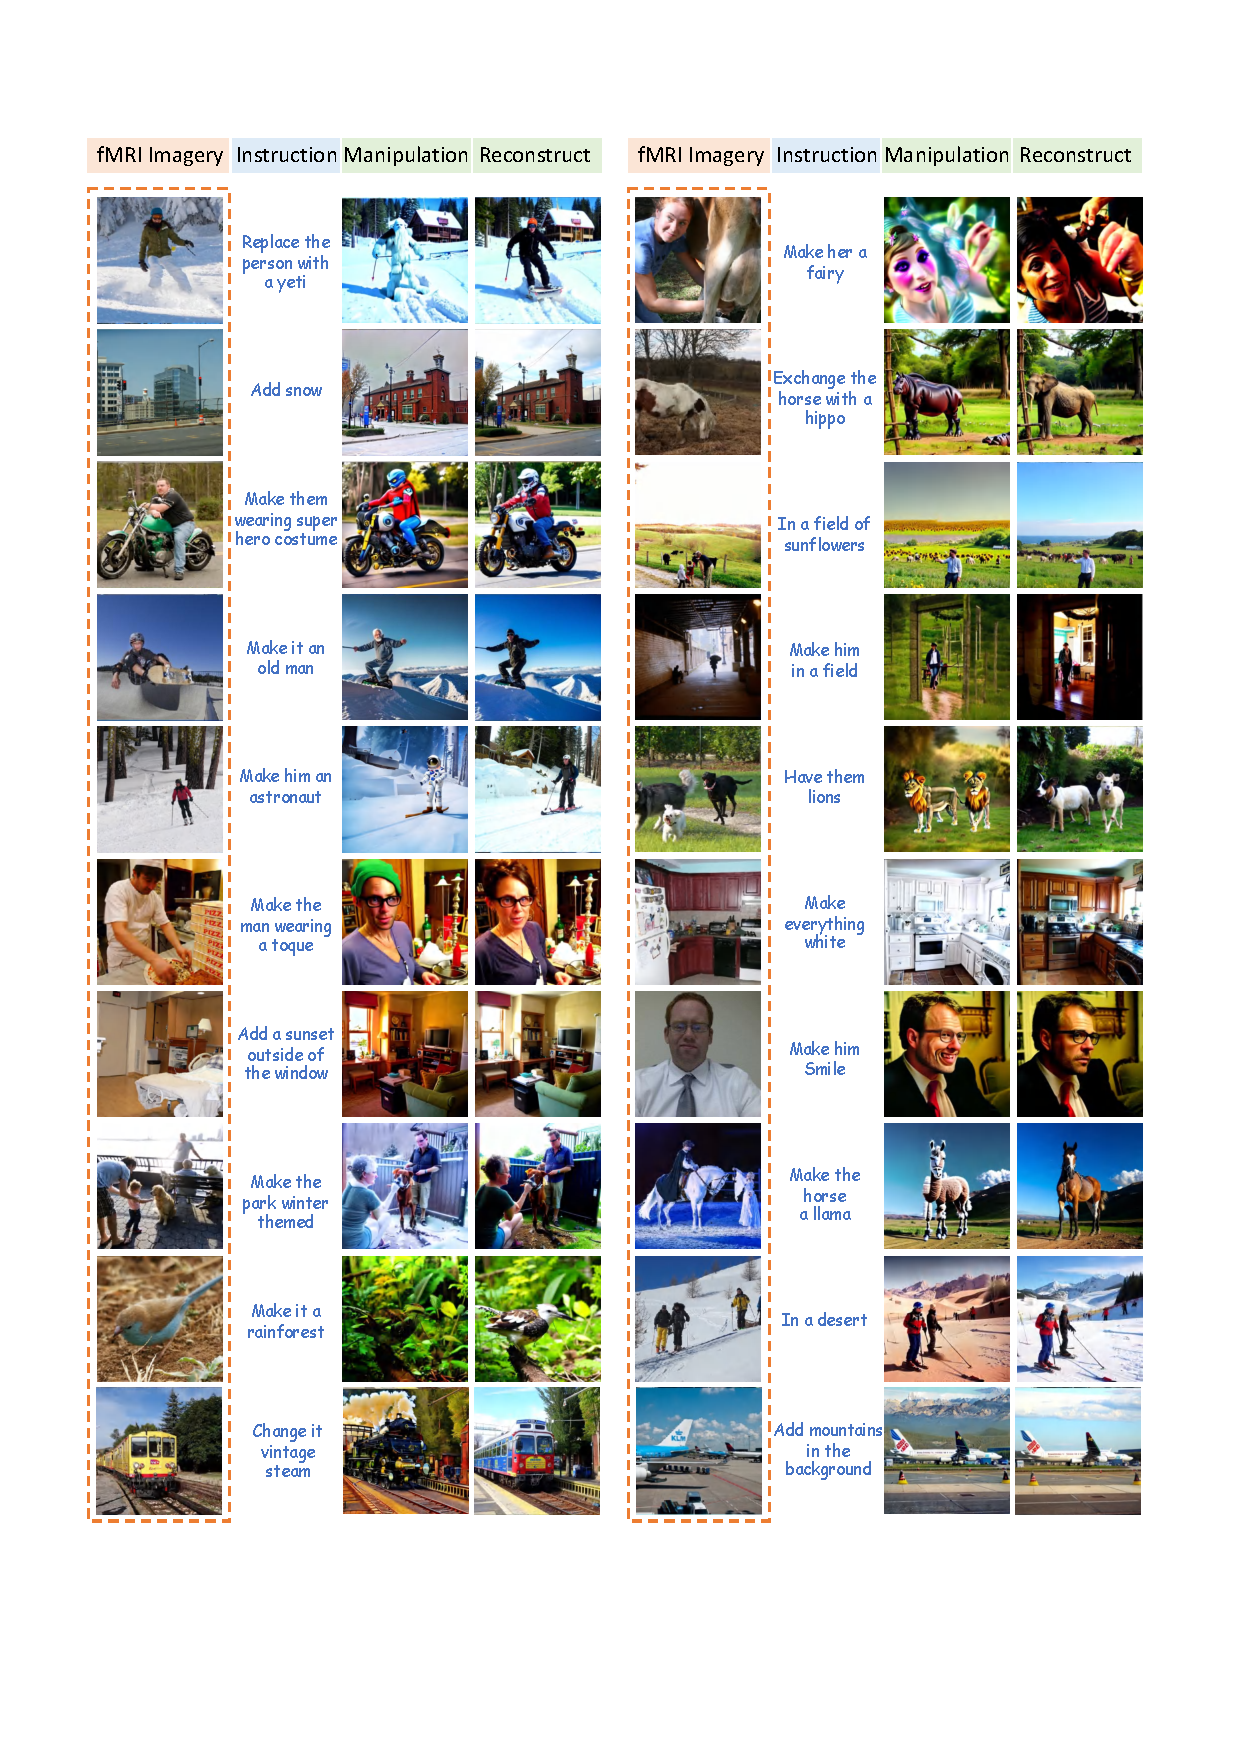
\includegraphics[width=1.0\textwidth]{figs/supp_edit0.pdf} 
    % \vspace{-4pt}
  \caption{\textbf{fMRI signal instruction with natural language description.} The first column displays the brain's visual stimulus. The second column illustrates the individual's intended operation. The third column presents the instruction results, while the fourth column shows the intermediate reconstruction results generated by our model.}
  \label{fig:supp_edit0}
  % \vspace{20pt}
\end{figure*}

\begin{figure*}[ht!]
  \centering
  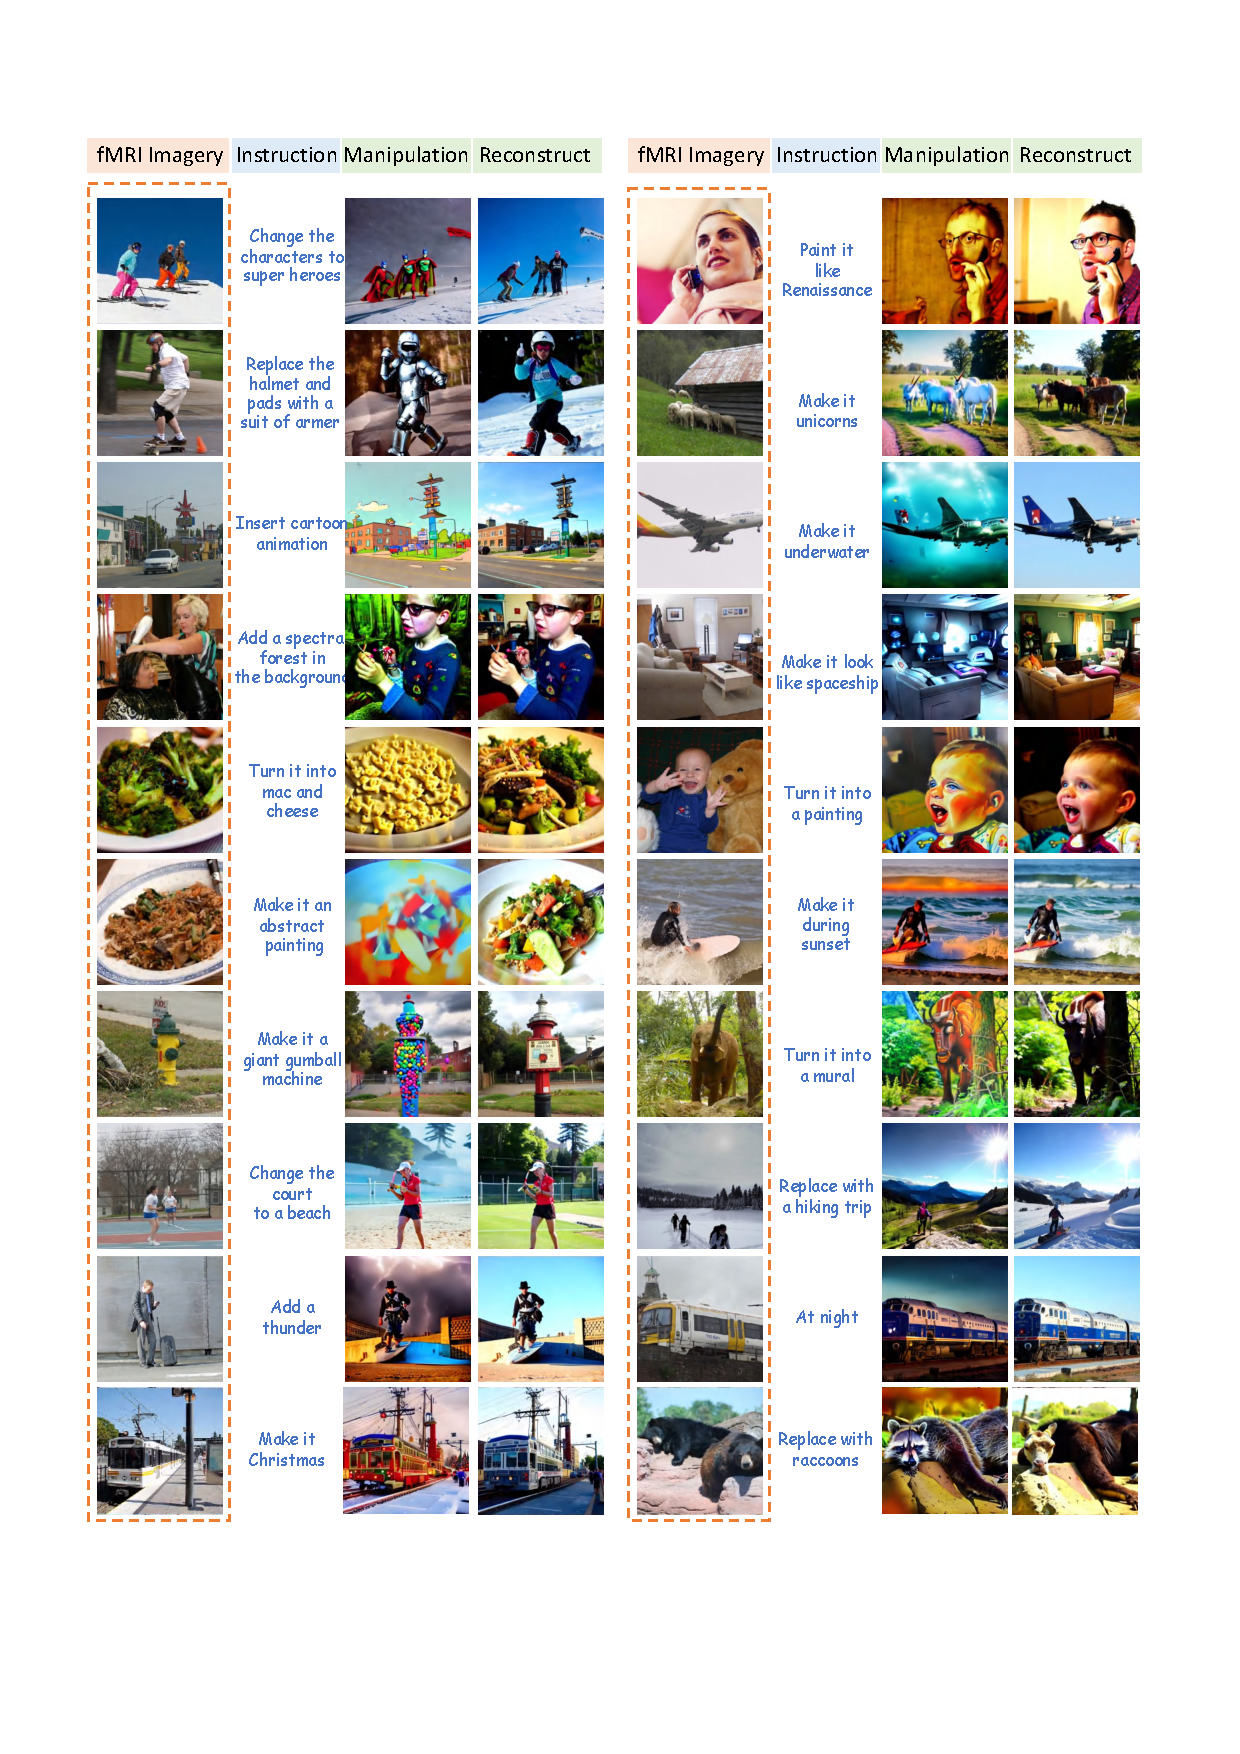
\includegraphics[width=1.0\textwidth]{figs/supp_edit1.pdf} 
    % \vspace{-4pt}
  \caption{\textbf{fMRI signal instruction with natural language description.} The first column displays the brain's visual stimulus. The second column illustrates the individual's intended operation. The third column presents the instruction results, while the fourth column shows the intermediate reconstruction results generated by our model.}
  \label{fig:supp_edit1}
  % \vspace{30pt}
\end{figure*}


\begin{figure*}[ht!]
  \centering
  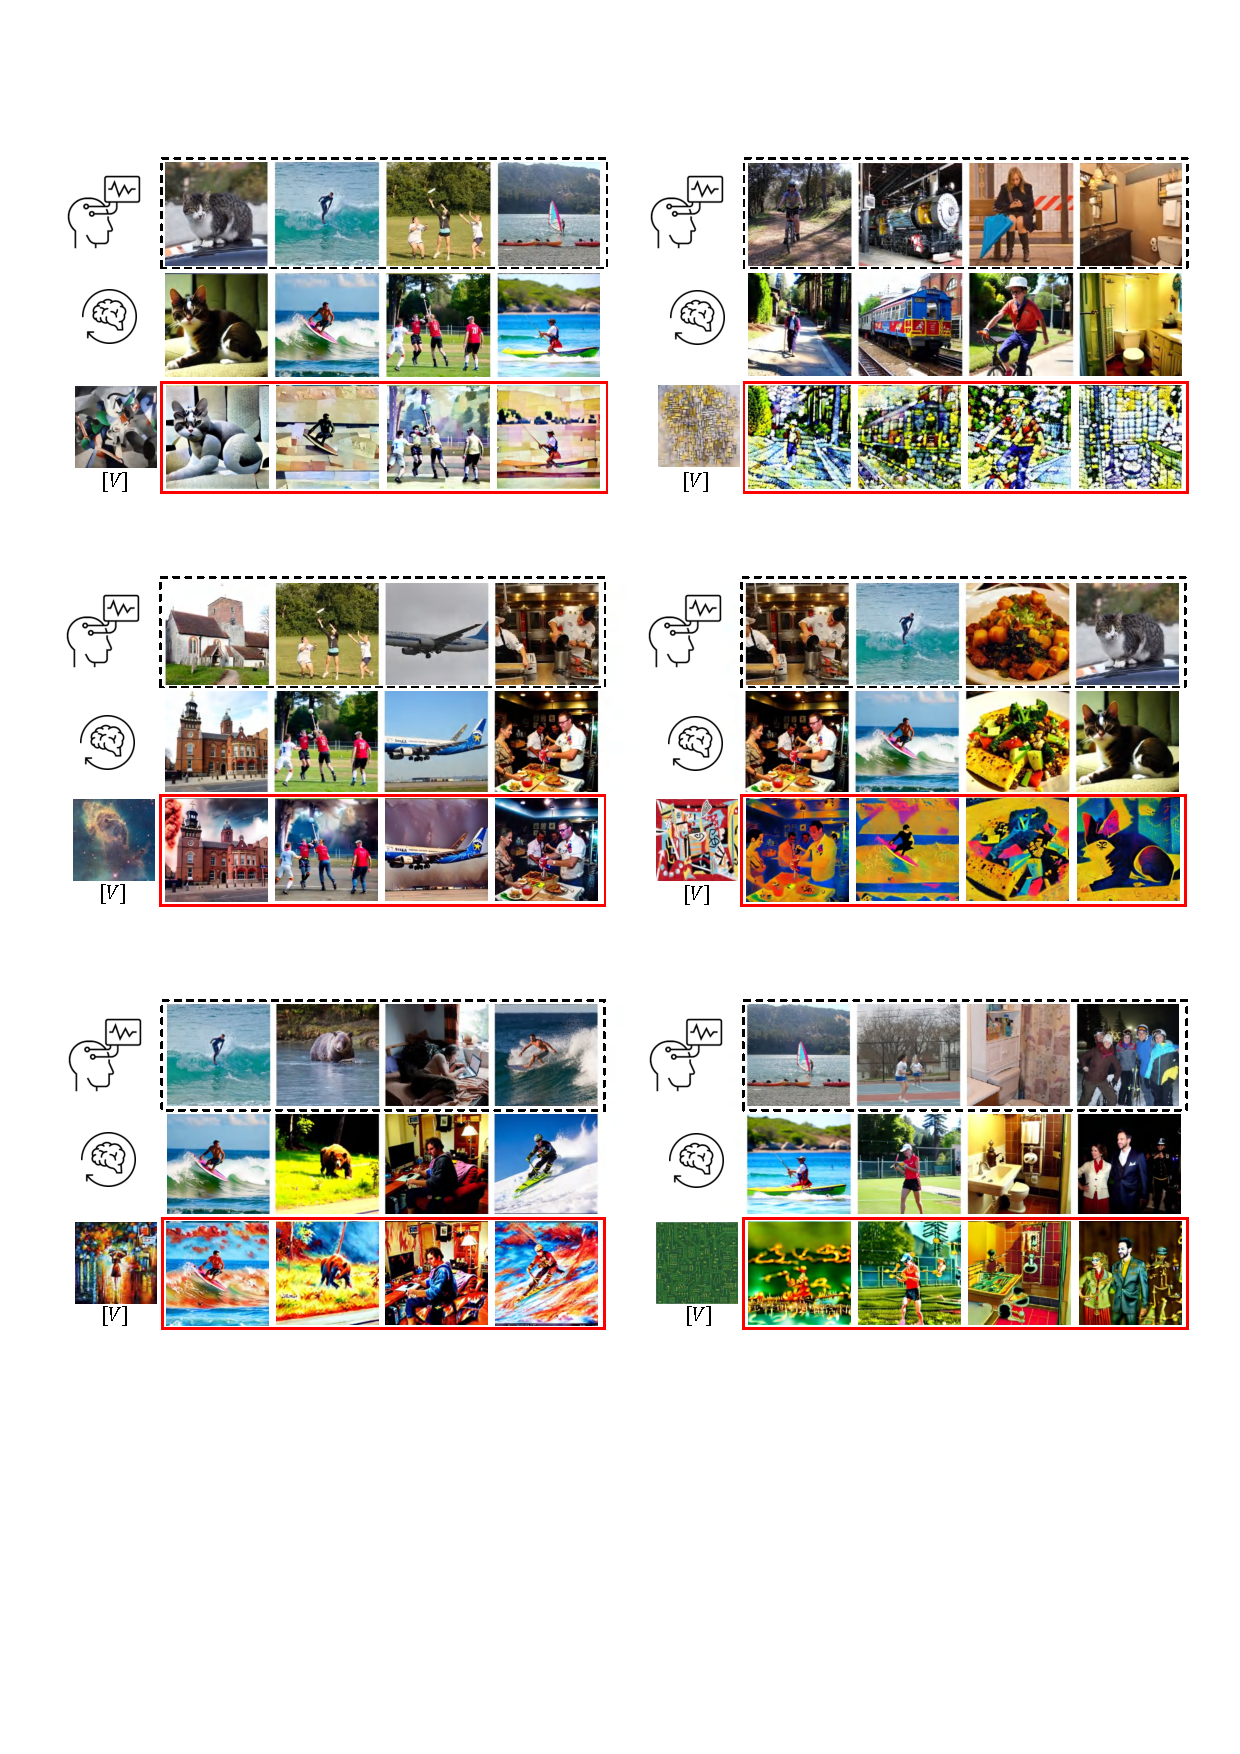
\includegraphics[width=1.0\textwidth]{figs/style_supp.pdf} 
    % \vspace{-4pt}
  \caption{\textbf{Demonstration Results of Multi-Modal Instruction.} First row list the visual stimulus while second row depict our intermediate reconstructions. The manipulation results via \emph{In the [V] style} are shown within red boxes of the last row.}
  \label{fig:supp_style}
  % \vspace{30pt}
\end{figure*}






% \begin{figure}[t!]
%   \centering
%   \includegraphics[width=0.98\textwidth]{figs/supp_results0.pdf} 
%     \vspace{-4pt}
%   \caption{\textbf{Image Manipulation Results by Visual Instruction.} }
%   \label{fig:supp_results0}
%   \vspace{-10pt}
% \end{figure}

\end{document}
